\documentclass[12pt, oneside]{Thesis}
\usepackage{palatino} 
\usepackage[utf8]{inputenc} 
\usepackage[T1]{fontenc}    
% The default font size and one-sided printing (no margin offsets)
\graphicspath{{Pictures/}}% Specifies the directory where pictures are stored
\usepackage[dvipsnames,svgnames,x11names,hyperref]{xcolor}
\usepackage[square, comma,  sort&compress]{natbib} % Use the natbib reference package - read up on this to edit the reference style; if you want text (e.g. Smith et al., 2012) for the in-text references (instead of numbers), remove 'numbers' 
\usepackage{tikz}
\usepackage{graphics}
\hypersetup{urlcolor=black, colorlinks=true, citecolor=blue, linkcolor=Black} % Colors hyperlinks in blue - change to black if annoying
\usepackage{lscape}
\usepackage{indentfirst}
\setlength{\parindent}{1cm}
%\usepackage{draftwatermark}
\usepackage{adjustbox}
\usepackage{tabularx}
\usepackage{float}
%\SetWatermarkScale{2}
%\SetWatermarkColor{red}
\usepackage{listings}
\usepackage{caption}
\captionsetup[lstlisting]{position=below}
\usepackage{color}
\usepackage{comment}
\usepackage{hyperref}
\usepackage{datetime}
\newdateformat{mydateformat}{\ordinaldate{\THEDAY} \monthname[\THEMONTH], \THEYEAR}

\definecolor{light-gray}{gray}{0.99}
\lstset{ language=python,% the language of the code
  numbers=left,% where to put the line-numbers
  numberstyle=\tiny\color{gray},% the style that is used for the line-numbers
  stepnumber=1,  % the step between two line-numbers. If it's 1, each line
   % will be numbered
  numbersep=5pt,  % how far the line-numbers are from the code
  backgroundcolor=\color{light-gray},% choose the background color. You must add \usepackage{color}
  showspaces=false,% show spaces adding particular underscores
  showstringspaces=false, % underline spaces within strings
  showtabs=false, % show tabs within strings adding particular underscores
  frame=single, % adds a frame around the code
  rulecolor=\color{JungleGreen},% if not set, the frame-color may be changed on line-breaks within not-black text (e.g. commens (green here))
  tabsize=2,  % sets default tabsize to 2 spaces
  captionpos=t, % sets the caption-position to top
  breaklines=true, % sets automatic line breaking
  breakatwhitespace=false, % sets if automatic breaks should only happen at whitespace
  title=\lstname, % show the filename of files included with \lstinputlisting;
 % also try caption instead of title
  keywordstyle=\color{RedViolet}, % keyword style
  commentstyle=\color{JungleGreen}, % comment style
  stringstyle=\color{Orange}, % string literal style
  escapeinside={\%*}{*}, % if you want to add a comment within your code
  aboveskip=0.4\baselineskip,
  belowskip=0.65\baselineskip,
  belowcaptionskip=10pt,
  morekeywords={*,...}% if you want to add more keywords to the set
} 
\definecolor{dkgreen}{rgb}{0,0.6,0}
\definecolor{gray}{rgb}{0.5,0.5,0.5}
\definecolor{navy}{rgb}{0,0,128}
\usepackage[dvipsnames]{xcolor}
\definecolor{antiquewhite}{rgb}{0.98, 0.92, 0.84}
\usepackage{longtable}
\usepackage{siunitx}
\sisetup{output-exponent-marker=\ensuremath{\mathrm{e}}}
\usepackage{fancyhdr}
\usepackage{multirow}
\usepackage{multicol}
\usepackage{enumitem}
\usepackage{caption}
\usepackage{tikz}



\setlength{\intextsep}{15pt}
\setlength{\abovecaptionskip}{0.7\baselineskip}
\setlength{\belowcaptionskip}{-1.2\baselineskip}
\setlist[itemize]{noitemsep, topsep=0pt}
\setlist[enumerate]{noitemsep, topsep=0pt}

%======================================================

% Define your custom macros for title, author, and supervisor
\def\ttitle{AI-Driven Medical Chatbot for Medical Students and Patients: An LLM and Embedding-Based Approach}
\def\authornames{Nataraju Tumakuru Shreeshylesha}
\def\supname{Prof. Dr. Chandna Swati}
\def\degreename{Master Of Science In Applied Data Science and Analytics}
\def\univname{SRH Hochschule Heidelberg}
\def\deptname{School of Information, Media and Design}
\def\subjectname{}
\def\keywordnames{}

% Title page setup
\title{\ttitle}

\begin{document}
\frontmatter % Use roman page numbering style (i, ii, iii, iv...) for the pre-content pages

\setstretch{1.3} % Set line spacing to 1.3

% Configure page headers and footers using the FancyHdr package
\fancyhead{} % Clear all page headers and footers
\rhead{\thepage} % Set the right side header to show the page number
\lhead{} % Clear the left side page header
\renewcommand{\footrulewidth}{0.1pt} % Set the width of the footer rule
%\rfoot{Your_name} % Uncomment and set the right footer text if needed
%\lfoot{} % Uncomment and set the left footer text if needed
\pagestyle{fancy} % Use the "fancy" page style to implement the FancyHdr headers

% Define a new command for a horizontal rule with a specific width
\newcommand{\HRule}{\rule{\linewidth}{0.5mm}}

% Set PDF meta-data using the hyperref package
\hypersetup{
    pdftitle={\ttitle}, % Set the PDF title
    pdfsubject=\subjectname, % Set the PDF subject
    pdfauthor=\authornames, % Set the PDF author
    pdfkeywords=\keywordnames % Set the PDF keywords
}

\begin{titlepage}
    \begin{center}
      
\includegraphics[width=6cm]{./Images/SRHLogo.png} % University/department logo - uncomment to place it

        \textsc{\LARGE \univname}\\[1.5cm] % University name
        \textsc{\Large Masters Thesis}\\[0.5cm] % Thesis type

        \HRule \\[0.4cm] % Horizontal line
        {\huge \bfseries \ttitle}\\[0.4cm] % Thesis title
        \HRule \\[1.5cm] % Horizontal line
        \large
        \emph{Author:}\\[0.2cm]
        \textsc{\authornames} % Author name

        \emph{Matriculation Number: 11027742} 
        %\vspace{0.5cm} % Add vertical space between author and supervisor sections

        \large
        \emph{Supervisors:} \\[0.2cm]
        \textsc{\supname} % Supervisor name

      
        \large \textit{A thesis submitted in fulfilment of the requirements for the degree of \\\degreename}\\[0.3cm] % University requirement text
        \textit{in the}\\[0.4cm]
        %\groupname\\

        \deptname\\[1.5cm] % Research group name and department name
        {\large \mydateformat\today}\\[1cm]  % Date
        

        \vfill
    \end{center}
  \end{titlepage}
%----------------------------------------------------------------------------------------
%	DECLARATION PAGE
%	Your institution may give you a different text to place here
%----------------------------------------------------------------------------------------

\Declaration{\vspace{1em}

I, \textbf{Nataraju Tumakuru Shreeshylesha}, declare that this thesis titled,  
\textit{“AI-Driven Medical Chatbot for Medical Students and Patients: An LLM and Embedding-Based Approach”}  
and the work presented in it is my own.  
I confirm that this work submitted for assessment is expressed in my own words and is my own.  
Any uses made within it of the works of other authors in any form (e.g., ideas, equations, figures, text, tables, programs)  
are appropriately acknowledged at any point of their use. A list of the references employed is included.

\begin{itemize}
\item[\tiny{$\blacksquare$}] This work was done wholly for a research degree at this University.
\item[\tiny{$\blacksquare$}] It has been clearly stated in this work if any part of this thesis has previously been submitted for a degree or any other qualification at this University or any other institution.
\item[\tiny{$\blacksquare$}] Where I have consulted the published work of others, credit is always given to the concerned work.
\item[\tiny{$\blacksquare$}] Where I have quoted from the work provided by others, the source is always given unless it is entirely my work.
\item[\tiny{$\blacksquare$}] I have acknowledged all main sources that supported me and helped during this work.
\end{itemize}

\vspace{2cm}
\noindent Signed:\\
\rule[1em]{25em}{0.5pt}

\noindent Date:\\
\rule[1em]{25em}{0.5pt}
}

\clearpage % Start a new page
%----------------------------------------------------------------------------------------
%	ACKNOWLEDGEMENTS
%----------------------------------------------------------------------------------------

\setstretch{1.3} % Reset the line-spacing to 1.3 for body text (if it has changed)
\acknowledgements{{\vspace{1em}} 

I am deeply grateful for the support and guidance of numerous individuals who have contributed to the completion of this thesis,  
and I would like to express my heartfelt appreciation to all of them. 

First and foremost, I would like to extend my sincere gratitude to my supervisor, Prof.Dr.Chandna Swati,  
for her invaluable guidance, expertise, and unwavering support throughout this research.  
Her mentorship has played a crucial role in shaping my ideas and refining my work.  

I am also grateful to the faculty and staff of the School of Information, Media and Design at SRH Hochschule Heidelberg  
for their continuous encouragement and for providing an enriching environment for research and learning.  

Special thanks to my colleagues and friends for their motivation, insightful discussions, and unwavering support.  
Their camaraderie has made this journey more fulfilling and enjoyable.  

I am profoundly indebted to my family for their unconditional love, patience, and encouragement throughout this journey.  
Their unwavering belief in me has been my greatest source of strength and perseverance.  

Lastly, I extend my gratitude to everyone who directly or indirectly contributed to the successful completion of this thesis.  
Your support and encouragement mean the world to me.  

}



\clearpage % Start a new page
\setstretch{1.1}
%\lhead{\emph{Abstract}} {\huge{\textit{Abstract}} \par}{{\vspace{1em}} 
\begin{abstract}{\vspace{1em}}
  \noindent Artificial intelligence (AI) is rapidly transforming the landscape of medical education and patient support. This thesis proposes an AI-driven medical chatbot system designed to serve two main user roles—medical students and patients—via distinct modes of operation. For medical students, the system provides an interactive knowledge platform with detailed explanations of complex topics, whereas for patients, it offers symptom analysis, healthcare provider recommendations, and even autonomous appointment booking through Agentic AI capabilities. 

  \noindent The architecture comprises several key components. First, textual data (such as PDFs of medical articles or learning materials) undergoes text extraction and chunking before being transformed into embeddings by a dedicated model. These embeddings are then indexed in a vector database, enabling efficient similarity-based retrieval. When a user submits a query, the system identifies and retrieves the most relevant text segments and subsequently augments the prompt for a Large Language Model (LLM), which can be tailored to specific roles: a learning AI assistant (e.g., Llama 2, 13B) for medical students and an agentic diagnostic AI (e.g., Mistral 13B) for patients. 

  \noindent In student mode, the chatbot focuses on explaining medical concepts and providing in-depth, evidence-based knowledge. In patient mode, the chatbot employs symptom analysis to generate preliminary diagnostic suggestions, seamlessly directing users to the HealthCare Provider Recommendation System. Harnessing its Agentic AI feature, the system can autonomously schedule appointments if necessary, reducing administrative overhead and expediting patient care. The entire process is orchestrated through a secure login mechanism, ensuring that only authorized users can access specific functionalities suited to their roles.

  \noindent Experimental evaluations draw upon real-world medical texts and feedback from both medical students and healthcare practitioners. Early results indicate that this approach effectively balances accurate medical guidance, educational depth, and practical utility in assisting patients. Future enhancements include expanding multi-language support, improving the LLM’s medical domain expertise, and integrating real-time health data streams to strengthen diagnostic accuracy.

\noindent\textbf{Keywords:} AI-driven Medical Chatbot, Role-based LLM, Patient Symptom Analysis, Healthcare Provider Recommendation, Autonomous Appointment Booking, Embedding Model, Vector Database

\end{abstract}


\clearpage % Start a new page

%----------------------------------------------------------------------------------------
%	LIST OF CONTENTS/FIGURES/TABLES PAGES
%----------------------------------------------------------------------------------------

\pagestyle{fancy} % The page style headers have been "empty" all this time, now use the "fancy" headers as defined before to bring them back

\lhead{\emph{Contents}} % Set the left side page header to "Contents"
\tableofcontents % Write out the Table of Contents

\lhead{\emph{List of Figures}} % Set the left side page header to "List of Figures"
\listoffigures % Write out the List of Figures

\lhead{\emph{List of Tables}} % Set the left side page header to "List of Tables"
\listoftables % Write out the List of Tables

\lhead{\emph{Listing of Sample Codes}}
\addtotoc{Listings}
\lstlistoflistings

\clearpage % Start a new page

%----------------------------------------------------------------------------------------
%	ABSTRACT PAGE
%----------------------------------------------------------------------------------------
\clearpage % Start a new page
%\addtotoc{Abstract} % Add the "Abstract" page entry to the Contents
%----------------------------------------------------------------------------------------
%	ABBREVIATIONS
%----------------------------------------------------------------------------------------

\clearpage % Start a new page

\setstretch{1.3} % Set the line spacing to 1.5, this makes the following tables easier to read

\lhead{\emph{Abbreviations}} % Set the left side page header to "Abbreviations"
\listofsymbols{ll} % Include a list of Abbreviations (a table of two columns)
{
\textbf{CTM} & \ Correlated Topic Model \\
\textbf{LDA} & \ Latent Dirichlet Allocation\\
\textbf{LSA} & \ Latent Semantic Analysis\\
\textbf{PLSA} & \ Probabilistic Latent Semantic Analysis\\
\textbf{NMF} & \ Non-Negative Matrix Factorization \\
\textbf{TF-IDF} & \ Term Frequency-Inverse Document Frequency  \\
\textbf{SVD} & \ Singular Value Decomposition  \\
\textbf{DBSCAN} & \ Density-Based Spatial Clustering of Applications with Noise \\
\textbf{HDBSCAN} & \ Hierarchical Density-Based Spatial Clustering of Applications with Noise \\
\textbf{HAC} & \ Hierarchical Agglomerative Clustering \\
\textbf{BERT} & \ Bidirectional Encoder Representations from Transformers \\
\textbf{NLP} & \ Natural Language Processing\\
\textbf{BIRCH} & \ Balanced Iterative Reducing and Clustering Hierarchies\\
\textbf{BOW} & \ Bag-of-words \\
\textbf{GloVe} & \ Global Vectors for Word Representation\\
\textbf{ML} & \ Machine Learning\\
\textbf{SBERT} & \ Sentence-Bidirectional Encoder Representations from Transformers\\
\textbf{GBERT} & \ German-Bidirectional Encoder Representations from Transformers\\
\textbf{T5} & \ Text-To-Text Transfer Transformer\\
\textbf{RoBERTa} & \ Robustly Optimized BERT\\
\textbf{UMAP} & \ Uniform Manifold Approximation and Projection\\
\textbf{PCA} & \ Principal Component Analysis\\
\textbf{T-SNE} & \ T-Distributed Stochastic Neighbor Embedding\\
\textbf{LLM} & \ Large Language Models\\
\textbf{GPT} & \ Generative Pre-trained Transformer\\
\textbf{LLaMA} & \  Large Language Model Meta AI\\
\textbf{JSON} & \ JavaScript Object Notation\\
}


%----------------------------------------------------------------------------------------
%	PHYSICAL CONSTANTS/OTHER DEFINITIONS
%----------------------------------------------------------------------------------------

%\clearpage % Start a new page

%\lhead{\emph{Physical Constants}} % Set the left side page header to "Physical Constants"

%\listofconstants{lrcl} % Include a list of Physical Constants (a four column table)
%{
%Speed of Light & $c$ & $=$ & $2.997\ 924\ 58\times10^{8}\ \mbox{ms}^{-\mbox{s}}$ (exact)\\

%% Constant Name & Symbol & = & Constant Value (with units) \\
%}

%----------------------------------------------------------------------------------------
%	DEDICATION
%----------------------------------------------------------------------------------------

%\setstretch{1.3} % Return the line spacing back to 1.3

%\pagestyle{empty} % Page style needs to be empty for this page

%\dedicatory{For/Dedicated to/To my\ldots} % Dedication text

%\addtocontents{toc}{\vspace{2em}} % Add a gap in the Contents, for aesthetics

%----------------------------------------------------------------------------------------
%	THESIS CONTENT - CHAPTERS
%----------------------------------------------------------------------------------------

\mainmatter % Begin numeric (1,2,3...) page numbering

\pagestyle{fancy} % Return the page headers back to the "fancy" style

\chapter{Introduction}

\label{Chapter1}
\section{Introduction}
Artificial Intelligence (AI) has become increasingly integral to modern healthcare and medical education, offering the promise of both better patient outcomes and more effective training for medical students. Traditionally, patient-facing solutions have relied on either rule-based systems or static information portals, often lacking deeper contextual understanding, adaptability, and the ability to perform autonomous tasks. Simultaneously, educational tools in medicine have mainly taken the form of passive content repositories or limited interactive platforms, providing a less-than-optimal experience for learning complex medical concepts.

\noindent This thesis addresses these limitations by proposing a role-based \textbf{AI-driven medical chatbot} capable of serving two distinct user groups:
\begin{itemize}
    \item \textbf{Medical Students:} An interactive learning environment where students can ask in-depth questions about medical topics and receive dynamic, evidence-based responses.
    \item \textbf{Patients:} A user-friendly interface for symptom assessment, healthcare provider recommendations, and automated appointment scheduling.
\end{itemize}

\noindent The system’s architecture harmonizes several advanced technologies:
\begin{enumerate}
    \item \textbf{Data Ingestion and Chunking:} Relevant medical texts (such as PDFs, articles, or curated training materials) are first broken into smaller, semantically coherent segments to facilitate granular retrieval and reduce extraneous information.
    \item \textbf{Embedding and Vector Storage:} Each chunk is converted into a numerical embedding via a specialized model (e.g., a general LLM-based encoder). These embeddings are then indexed in a \emph{vector database}, allowing high-speed similarity searches to quickly identify the text segments most relevant to a user’s query.
    \item \textbf{Retrieval-Augmented Generation (RAG):} When a user submits a query, the system retrieves the top-matching chunks from the vector database. The large language model (LLM) then leverages these retrieved segments as context, enhancing the accuracy and trustworthiness of its generated responses.
    \item \textbf{Role-based Large Language Models:} The chatbot differentiates between “student mode” (providing detailed medical knowledge and conceptual explanations) and “patient mode” (offering symptom-based advice and potential next steps). This role-specific approach ensures \emph{in-depth} responses for students and \emph{accessible} guidance for patients.
    \item \textbf{Agentic AI for Appointment Booking:} The system integrates an \emph{agentic} component that allows it to autonomously schedule or reschedule appointments. This feature reduces administrative overhead for providers and streamlines patient journeys, potentially leading to faster access to care.
\end{enumerate}

\noindent The proposed chatbot thus spans a wide range of capabilities—from deep academic support for medical students to practical, real-world patient solutions. By uniting \emph{embedding-based retrieval}, \emph{role-aware LLMs}, and \emph{autonomous scheduling}, the architecture tackles existing gaps in both user groups’ experiences: medical students gain a dynamic tutor that can recall and contextualize complex material, while patients receive an accessible, on-demand assistant that not only provides preliminary information but also handles logistical tasks like finding the right specialist and booking an appointment.

\noindent Furthermore, ensuring a robust, user-centric design requires addressing core challenges. These include:
\begin{itemize}
    \item \textbf{Data Quality and Scope:} The medical knowledge base must be reliable, up-to-date, and appropriately chunked to avoid misinformation.
    \item \textbf{Model Accuracy and Safety:} Large language models can exhibit “hallucination” or produce erroneous conclusions; thus, retrieval of verifiable source chunks is critical.
    \item \textbf{Ethical and Regulatory Considerations:} Patient data privacy, informed consent, and adherence to healthcare regulations remain paramount, particularly in managing personal health information and scheduling details.
    \item \textbf{User Experience Across Roles:} The interface must distinguish clearly between student and patient usage, providing advanced conceptual detail to students while simplifying medical jargon for patients.
\end{itemize}

\noindent Through systematic experimentation, including real-time feedback from both students and healthcare providers, this thesis evaluates the effectiveness of the proposed chatbot architecture in meeting these goals. The subsequent chapters detail the underlying technologies, design methodologies, system evaluation metrics, and future enhancements that together shape an advanced, \emph{role-based} AI solution for bridging medical education and patient-centric healthcare. 


% ============================================================================
% section : motivation
% =============================================================================
\section{Motivation}
\label{sec:motivation}

Modern healthcare simultaneously faces escalating patient demands and a persistent shortage of medical professionals. On one hand, patients often require immediate attention and convenient scheduling mechanisms to mitigate anxiety, enhance treatment adherence, and reduce missed diagnoses. On the other hand, medical students and early-career clinicians must navigate the complexities of specialized knowledge, hands-on practice, and ever-evolving guidelines to stay current. Traditional educational methods—such as static textbooks and passive lectures—can be inadequate for preparing learners to handle complex, real-time scenarios.

\noindent In parallel, conventional patient-facing tools, such as basic symptom checkers or rule-based triage systems, rarely provide sufficient context or personalized guidance. They also lack direct integration with hospital resources for scheduling appointments. Consequently, patients may feel uncertain about the seriousness of their symptoms or spend valuable time consulting multiple, unverified online sources.

\noindent These challenges point toward a critical need for a comprehensive solution that offers:
\begin{itemize}
    \item \textbf{On-demand access to credible information:} 
    For patients, this means efficient triage and clarity regarding symptoms. For students, it entails interactive learning tools that simulate realistic, complex queries.
    \item \textbf{Reduced administrative barriers:} 
    Automating tasks like appointment booking frees up health professionals’ time and ensures that patients receive timely care. 
    \item \textbf{Seamless retrieval of validated data:} 
    Whether it is up-to-date medical guidelines or localized healthcare provider information, the system must unify relevant data and present it contextually. 
    \item \textbf{Adaptability for different user roles:}
    Advanced question-answering for students differs substantially from straightforward symptom analysis and scheduling for patients. A single chatbot must fluidly handle these distinct modes.
\end{itemize}

\noindent By harnessing \emph{large language models (LLMs)}, advanced embedding-based \emph{retrieval systems}, and \emph{agentic} AI capable of autonomously interacting with scheduling APIs, it becomes possible to unify medical education and patient-centric services in a single platform. This unified approach promises immediate benefits:
\begin{enumerate}
    \item \textbf{Enhanced Learning:} Students can query the system at any complexity level, receiving deep, evidence-based explanations and case scenarios, thus bridging the gap between theoretical knowledge and real-world clinical encounters.
    \item \textbf{Better Patient Outcomes:} Prompt appointment booking and symptom clarity can reduce treatment delays, lowering the risk of complications and alleviating patient stress.
    \item \textbf{Administrative Efficiency:} Automated booking workflows diminish the overhead for healthcare facilities, reducing staff workload and the chance of scheduling errors or gaps.
\end{enumerate}

\noindent Ultimately, the motivation for developing this dual-mode medical chatbot is to transcend the limitations of single-purpose educational platforms or simplistic symptom checkers. Instead, an \textbf{integrated AI-driven framework} is poised to deliver tailored user experiences, ensure seamless data flow, and cultivate both improved healthcare accessibility for patients and a transformative learning ecosystem for medical students.

% ============================================================================
% section : problem statement
% =============================================================================
\vspace{2cm}
\section{Problem Statement and Challenges}
\label{sec:problem-statement}

Two problems define modern healthcare: patients require consistent counsel when faced with conflicting symptoms; medical students need basic access to current, accurate material to improve their core knowledge and prepare ready for clinical practice. Often missing the timeliness, complexity, and contextual clarity needed for complicated medical situations are existing solutions such simple symptom checklists or static web-based services. Furthermore, these stand-alone technologies seldom provide for timely scheduling or referral, thus leaving patients wondering about their next line of action on their medical route.

With regard to medical students especially, the difficulty is in Five Short Notes Names Especially when doing so in real time or when referencing other disciplines (pharmacy and pathology, for example), negotiating enormous numbers of research articles, medical textbooks, and clinical case reports can be challenging. Conventional e-learning systems barely combine theoretical knowledge with practical, scenario-based learning and lack efficient Q\&A systems that fit to user inquiries.

\noindent \textbf{Timeliness and Accuracy:} Medical technology is evolving so rapidly that conventional resources could soon become extinct. Students run the danger of picking out outdated methods without fast, current sources.

About the patients, the challenges are equally important: Deciding whether their symptoms call for frequent visits or urgent care can be challenging for people, which could lead to worry and maybe postpone treatment.

\noindent \textbf{Obstacles blocking healthcare access:} Usually involving many phone calls or internet searches, making an appointment with a specialist or follow-up visit delays patients from receiving proper treatment---especially those unclear of the sort of expert to see.

\noindent \textbf{Unverified or contradicting information:} Patients may be pushed to self-diagnose via questionable online sources as basic symptom-checking websites may be inadequate or non-personalized.

Thus, the main challenge is designing a single, synthetic intelligence-powered system that satisfies both sets of needs:
\begin{enumerate}
    \item A comprehensive teaching tool for medical students responding in-depth, contextually sensitively to specific questions derived from properly chosen clinical and scholarly sources. Allays any concerns, rapidly links patients to pertinent medical experts, and offers initial direction based on a patient-facing symptom analysis and triage mechanism.
    \item Agentic appointment management helps to reduce administrative load and fill the information gap between pragmatic healthcare measures by enabling the system autonomously organize or postpone patient appointments. 
\end{enumerate}

These underlines the requirement of including Large Language Models (LLMs), embedding-based data retrieval, and user role-aware interactions. One such strategy is: Abbreviations 6 covers the academic demands needed for medical school as well as the pragmatic, immediate concerns patients have when presented with health issues. The next parts will address how this integrated chatbot idea may provide medical students and patients accurate, ethically acceptable, contextually relevant advice.


% ============================================================================
% section : research questions
% =============================================================================

\section{Research Questions}
To answer the problem statements, following research questions needs to be answered.
Below-mentioned research questions are obtained from the above-mentioned problem statements.

\noindent\textbf{Research question 1: }  
Does topic modelling aid in the extraction of topic process from the dataset of past interviews?

\noindent The best topic modelling techniques for extracting topics from the dataset must be analyzed to answer 
this research issue, which calls for a review of the literature.

\noindent\textbf{Research question 2: }
How can we use various clustering techniques to extract information and cluster them from the German dataset?

\noindent Different types of clustering algorithms must be understood by reading through the literature to 
choose which algorithm is most suited for completing the work at hand. This question will provide to understand 
and chose the right algorithm.

\noindent\textbf{Research question 3: }
How can language models be applied for topic modelling of German datasets?

\noindent Finding language models that perform well in German frequently requires a careful reading through many research articles that cover 
multilingual models or models created especially for German text.
% ============================================================================
% section : Thesis Structure
% =============================================================================
\vspace{10cm}
\section{Thesis Structure}

This section will provide an overview and also explain the structure about the chapters which will be covered as part of the thesis:

Chapter 2 gives a broad overview of state-of-the-art methodologies which will help to understand the various techniques which are
 used in past to overcome the issue and the technique used for implementation of the thesis. Each of these methodologies is 
 meticulously elucidated, offering a thorough understanding of their application and significance.

Chapter 3 explains about the thesis implementation pipeline, providing a comprehensive overview of each step included
 within the thesis framework. In this chapter, short explanations for every component of the thesis implementation process
  are also discussed.

Chapter 4 focuses on the practical implementation phase, were essential libraries are mentioned and gain a comprehensive understanding
 of the models employed to accomplish our task. This chapter provides a thorough breakdown of the libraries utilized throughout the 
 code, specifying their roles in different sections of the code.

Chapter 5 is about the evaluation of the methodologies used to evaluate the cluster formation and topic extraction. 
It explains about the performance of  the models and talks about the best performing model.

Chapter 6 is the final chapter and will provides the thesis conclusion and mention some of the challenges faced during
the implementation of thesis along with the ideas on how the model can be improved and which other LLM models can be used
as a part of the future work.
\chapter{State-of-the-Art}

\section{Introduction}
The confluence of advanced artificial intelligence, massive data availability, and evolving clinical needs has transformed healthcare and medical education. In recent years, large language models (LLMs) and sophisticated embedding techniques have emerged as transformative tools that enable dynamic patient engagement and interactive educational support. These technologies now underpin conversational systems capable of handling complex, unstructured clinical data and generating contextually nuanced responses. This chapter provides an exhaustive review of the state-of-the-art approaches in the field, covering historical developments, technical innovations, decentralized data architectures, and evaluation methodologies. By integrating insights from two pivotal studies—Paper~1 and Paper~2—we lay the foundation for our dual-mode architecture designed to support both medical students and patients.

Our review is organized into several sections. Section~2.2 surveys the literature and traces the evolution of LLMs in healthcare; Section~2.3 delves into the methodologies, including retrieval-augmented generation, advanced embedding, dimensionality reduction, and clustering techniques; Section~2.4 addresses decentralized architectures and privacy-enhancing technologies; Section~2.5 outlines evaluation strategies and benchmarks; and Section~2.6 discusses the system architectures that support these functionalities. We conclude with Section~2.7, which explores the challenges and future research directions.

\section{Literature Review}

\subsection{Evolving Role of LLMs in Healthcare and Medical Education}
Historically, early healthcare information systems relied on rule-based expert systems and static databases with limited adaptability. With the advent of statistical language models and later deep learning approaches, the focus shifted toward data-driven methods. The introduction of transformer architectures in 2017 revolutionized natural language processing (NLP) by enabling models such as BERT and GPT to capture long-range dependencies and contextual nuances. This transformation paved the way for models that could generate highly fluent and context-sensitive responses.

Recent breakthroughs—exemplified by GPT-4 and open-source models like Meta’s LLaMa series—have unlocked new possibilities for both clinical decision support and medical education. Paper~2 demonstrates that LLMs can now generate patient-tailored dialogue and educational content with remarkable fluency. However, both papers note that such systems require careful domain-specific adaptation and robust retrieval mechanisms to ensure factual accuracy.

\subsection{Decentralized Architectures for Data Privacy}
Data privacy is a critical concern in healthcare. Traditional centralized systems are vulnerable to data breaches and unauthorized access, posing significant regulatory and ethical challenges. Paper~1 proposes a decentralized architecture using Personal Data Stores (PDS) coupled with blockchain-based access controls. This approach empowers patients to maintain control over their own data while granting secure, auditable access to healthcare providers. Such architectures are designed to comply with stringent regulations (e.g., GDPR, HIPAA) and mitigate the risks inherent in centralized data storage.

Decentralization not only enhances data security but also builds trust among users. By filtering and de-identifying sensitive information at the edge before processing by LLMs, these architectures ensure that clinical interactions remain both private and effective.

\subsection{Conversational AI for Patient Engagement and Education}
Recent research has demonstrated the transformative potential of conversational AI systems in healthcare. Paper~2 outlines a multi-layered conversational framework where patient inputs are first processed by specialized modules—ranging from ad-hoc parsers for vital signs to intent recognition systems (e.g., Wit.AI)—before being passed to an LLM for free-form dialogue. This tiered approach is designed to protect sensitive clinical data while enabling rich, empathetic interactions.

For medical students, similar systems provide interactive tutoring that offers in-depth, evidence-based explanations and simulates realistic clinical scenarios. Tailoring responses based on user roles significantly enhances the system’s utility, meeting the divergent needs of patients and students.

\subsection{Methodological Innovations in Topic Modelling and Information Retrieval}
Traditional topic modelling methods such as Latent Dirichlet Allocation (LDA), Non-negative Matrix Factorization (NMF), and Probabilistic Latent Semantic Analysis (PLSA) rely on bag-of-words representations, which often fail to capture the context-dependent meaning of medical texts. Recent innovations integrate deep learning-based embeddings and neural topic models (e.g., BERTopic) to extract more semantically rich topics.

Both Paper~1 and Paper~2 highlight the use of retrieval-augmented generation (RAG) as a means to ground the generative process in verifiable sources. By indexing trusted medical texts in a vector database and retrieving contextually relevant passages, these approaches improve both accuracy and reliability in clinical applications.

\section{Methodologies}

\subsection{Retrieval-Augmented Generation (RAG)}
Retrieval-Augmented Generation (RAG) combines robust retrieval systems with powerful generative models to produce responses that are both fluent and factually accurate. In this approach, a vector database is populated with embeddings derived from a corpus of trusted medical literature (e.g., clinical guidelines and peer-reviewed articles). When a query is received, the retrieval system identifies the most relevant document fragments, which are then provided as context to the LLM.

This integration helps to mitigate hallucination by anchoring responses in verified data while enhancing the contextual richness of the generated responses. Both Paper~1 and Paper~2 provide evidence that RAG frameworks significantly improve the reliability of chatbot systems in healthcare.

\subsection{Advanced Embedding Techniques}
Embeddings convert text into dense numerical vectors that capture semantic meaning. Early methods such as Word2Vec and GloVe laid the groundwork, but transformer-based approaches like Sentence-BERT now dominate due to their ability to incorporate contextual cues. For multilingual and domain-specific applications—especially for German clinical texts—models such as GBERT, Cross English \& German RoBERTa, and Jina embedding-v2-base-de are employed.

These embeddings are further refined using dimensionality reduction techniques such as UMAP, which projects high-dimensional vectors into lower-dimensional spaces while preserving intrinsic semantic relationships.

\subsection{Dimensionality Reduction and Clustering}
Dimensionality reduction is essential to manage high-dimensional embeddings. Techniques such as PCA, t-SNE, and UMAP reduce computational complexity and facilitate visualization. UMAP is particularly favored for its ability to preserve local and global data structures.

After reduction, clustering algorithms like HDBSCAN are applied to group semantically similar texts. HDBSCAN is preferred over methods like K-Means due to its robustness against noise and its ability to automatically determine the number of clusters. This multi-stage pipeline—embedding, dimensionality reduction, clustering, and topic extraction via LLMs—forms the backbone of modern topic modelling systems in digital health.

\subsection{Topic Extraction via LLMs}
Once clusters are formed, each group of semantically similar texts is processed to generate a concise topic label. An LLM (e.g., Llama 3.1) is used to synthesize information from each cluster and generate a topic name that captures the core theme. This process, driven by prompt engineering, enables the extraction of meaningful, context-aware topics, outperforming traditional bag-of-words methods.

\subsection{Integrated System Architecture}
Our proposed system architecture is highly modular and layered. It consists of:
\begin{itemize}
    \item \textbf{Data Ingestion and Preprocessing:} Raw data from clinical texts, patient inputs, and educational materials are cleaned, segmented, and tokenized.
    \item \textbf{Embedding Generation and Storage:} Advanced embedding models convert the preprocessed text into dense vectors, which are stored in a vector database.
    \item \textbf{Retrieval Module:} Upon receiving a query, the system retrieves contextually relevant document fragments using similarity metrics.
    \item \textbf{Generative Module:} A fine-tuned LLM processes the query and retrieved context to generate a response.
    \item \textbf{Role-Aware Adaptation:} The system dynamically adjusts its response style based on whether the interaction is with a patient or a medical student.
    \item \textbf{Decentralized Data Management:} Sensitive patient data are managed via Personal Data Stores (PDS) and blockchain-based access controls.
    \item \textbf{Agentic Functionality:} Additional modules enable automated tasks such as appointment scheduling and real-time reminders.
\end{itemize}

Figure~\ref{fig:architecture} illustrates the overall system architecture. This diagram, adapted from the architectures presented in Paper~1 and Paper~2, visually summarizes the flow from data ingestion to LLM-based response generation.


\section{Challenges}

\subsection{Factual Accuracy and Mitigating Hallucination}
LLMs are known to occasionally generate plausible yet factually incorrect responses (hallucinations). This risk is especially critical in healthcare, where inaccuracies can lead to severe consequences. While RAG helps ground responses in verified data, ensuring that the retrieval module consistently provides comprehensive and current context remains challenging. Future work must explore dynamic knowledge updating and domain-specific fine-tuning to further mitigate these issues.

\subsection{Data Privacy, Security, and Ethical Considerations}
Handling sensitive medical data demands stringent privacy and security measures. Decentralized architectures and data de-identification techniques, as outlined in Paper~1, are promising but require careful balancing to maintain data utility. Ethical concerns, including transparency, bias mitigation, and informed consent, are also paramount. Developing robust data governance and auditing frameworks is essential for building trust and ensuring regulatory compliance.

\subsection{Computational and Resource Constraints}
The computational demands of LLMs and high-quality embedding models are substantial. Processing large volumes of clinical data in real time requires significant GPU resources, memory, and processing power. Optimization strategies—such as model compression, quantization, and efficient batch processing—are necessary to reduce resource consumption and enable scalable deployments.

\subsection{Complexity in Evaluation and Benchmarking}
Evaluating AI systems in healthcare is inherently complex due to the need to balance automated quantitative metrics with qualitative human judgment. While metrics such as semantic similarity, precision@k, and clustering indices provide useful insights, they cannot fully capture aspects such as empathy, clarity, and clinical relevance. Standardizing evaluation protocols that integrate both automated and human-centric assessments remains an ongoing research challenge.

\section{Evaluation Strategies}

\subsection{Quantitative Metrics}
A comprehensive evaluation employs multiple quantitative metrics:
\begin{itemize}
    \item \textbf{Semantic Similarity Scores:} Cosine similarity measures the closeness between generated responses and gold-standard references.
    \item \textbf{Retrieval Metrics:} Metrics like Precision@k and Mean Reciprocal Rank (MRR) assess the effectiveness of the retrieval module.
    \item \textbf{Clustering Validity Indices:} Silhouette Score, Davies-Bouldin Index, and Calinski-Harabasz Index evaluate the coherence and separation of clusters.
    \item \textbf{Pairwise Comparison:} Advanced methods utilize expert LLMs (e.g., GPT-4) to compare outputs across dimensions such as relevance, coherence, and fluency.
\end{itemize}

\subsection{Human-Centric Evaluations}
In addition to quantitative metrics, human evaluations are crucial:
\begin{itemize}
    \item \textbf{User Studies and Surveys:} Collect feedback from clinicians, patients, and medical students regarding clarity, empathy, and clinical relevance.
    \item \textbf{Expert Panels:} Engage healthcare professionals to assess the accuracy and utility of the chatbot’s outputs.
    \item \textbf{Task-Based Evaluations:} Design real-world clinical scenarios and educational simulations to evaluate system performance.
    \item \textbf{Longitudinal Studies:} Monitor user satisfaction and system performance over time to evaluate long-term impact.
\end{itemize}

\subsection{Comparative Benchmarking}
Comparative studies are essential to contextualize performance:
\begin{itemize}
    \item \textbf{Traditional vs. Modern Approaches:} Benchmark the LLM-based approach against conventional methods (e.g., LDA, NMF).
    \item \textbf{Cross-Model Evaluations:} Compare outputs from different LLMs (e.g., GPT-3.5, Llama2-70B, Mistral-7B) under identical conditions.
\end{itemize}

\section{System Architectures}

\subsection{Decentralized Data Architectures and Personal Data Stores (PDS)}
Paper~1 proposes a decentralized data architecture that employs Personal Data Stores (PDS) in conjunction with blockchain-based smart contracts. This design empowers patients by ensuring that sensitive data remain under their control and only accessible by authorized healthcare providers. Such an approach minimizes the risks of centralized data breaches and complies with regulatory frameworks like GDPR and HIPAA. The decentralized model further supports traceability and transparency, essential for ethical data governance.

\subsection{Modular and Layered Conversational Frameworks}
Effective LLM-based chatbot systems are designed using a modular, layered approach:
\begin{itemize}
    \item \textbf{Input Processing:} Raw data are preprocessed, cleaned, and segmented to remove noise.
    \item \textbf{Embedding and Retrieval:} Advanced embedding models transform text into dense vectors that are stored in a vector database for efficient retrieval.
    \item \textbf{Generative Response:} An LLM processes the query together with the retrieved context to generate a role-specific response.
    \item \textbf{Decentralized Management:} Sensitive data are managed via decentralized architectures to ensure privacy.
    \item \textbf{Agentic Functionality:} Automated modules facilitate tasks such as appointment scheduling.
\end{itemize}

\subsection{Integration of RAG within a Secure, Decentralized Framework}
The integration of Retrieval-Augmented Generation (RAG) within a decentralized framework is a key innovation. By retrieving context from verified sources and ensuring that only de-identified data are processed by the LLM, the system achieves both factual accuracy and data security. This integration is critical for applications in healthcare, where both accuracy and privacy are paramount.

\section{Future Directions}

\subsection{Enhancing Model Reliability and Factual Accuracy}
Future research must address the challenges of reducing hallucination and ensuring factual accuracy by:
\begin{itemize}
    \item Implementing domain-specific fine-tuning.
    \item Integrating hybrid verification systems.
    \item Developing dynamic knowledge updating mechanisms.
\end{itemize}

\subsection{Expanding Privacy, Security, and Ethical Frameworks}
Advancements in privacy-enhancing technologies such as federated learning, differential privacy, and secure multi-party computation are essential. Establishing transparent data governance and bias mitigation strategies will further enhance ethical compliance.

\subsection{Overcoming Computational and Scalability Constraints}
To manage increasing computational demands, future systems should focus on:
\begin{itemize}
    \item Resource-efficient architectures through model compression and quantization.
    \item Distributed computing strategies using scalable cloud and edge infrastructures.
    \item Optimized batch processing to reduce runtime.
\end{itemize}

\subsection{Integrating Multimodal and Cross-Domain Capabilities}
The next generation of healthcare chatbots will benefit from:
\begin{itemize}
    \item Multimodal fusion of text, images, sensor data, and structured clinical records.
    \item Cross-domain adaptation to seamlessly transition between clinical decision support and educational tutoring.
    \item Cultural and linguistic adaptation to serve diverse populations effectively.
\end{itemize}

\subsection{Standardizing Evaluation Protocols}
There is a pressing need to develop standardized evaluation frameworks that integrate both quantitative metrics and human-centric assessments. Future work should focus on:
\begin{itemize}
    \item Creating integrated benchmarking protocols.
    \item Conducting longitudinal studies to evaluate long-term impact.
    \item Fostering interdisciplinary collaboration to refine evaluation standards.
\end{itemize}

\section{Summary}
This chapter has provided an exhaustive review of the state-of-the-art in LLM-driven systems for healthcare and medical education. We traced the evolution of LLMs from early transformer models to modern systems that offer advanced fluency and contextual understanding. Detailed discussions on retrieval-augmented generation, advanced embedding techniques, dimensionality reduction, and robust clustering methodologies were presented, along with an in-depth analysis of decentralized architectures and privacy-enhancing techniques as outlined in Paper~1. Comprehensive evaluation strategies that blend automated metrics with human assessments were also discussed, highlighting the strengths and limitations of current systems.

The multi-layered system architecture—combining data ingestion, embedding generation, retrieval, and LLM-driven response generation—forms the foundation for our proposed dual-mode system. By addressing critical challenges such as factual accuracy, data privacy, computational efficiency, and evaluation complexity, our thesis aims to bridge the gap between clinical practice and medical education.

Future research directions include enhancing model reliability, integrating multimodal data sources, expanding decentralized frameworks, and standardizing evaluation protocols. These efforts will be essential for developing next-generation AI-driven medical chatbots that improve patient engagement and educational outcomes.

\clearpage
 
\chapter{Design and Methodology}

\label{Chapter3}

\lhead{Chapter 3. \emph{Design and Methodology}}

This chapter is about the blueprint and the Methodologies used in the thesis involves a systematic progression of 
the steps to ensure a careful exploration of the topic modelling techniques. The process contains various steps and the implementation 
will start from the point of data collection and then analysing the data leading to the interpretation of results and their 
alignment with the initial research objective. The collected data is analysed then transformed into a format that is conductive
for the effective processing which involves few steps like removal of unwanted data, combining the data, cleaning the data, and 
so on then, the data is used to feed into the model to obtain the results. Finally, the thesis concludes with a discussion
of findings, implications, and potential avenues for future research, presenting a well-rounded culmination of the research endeavour.
Figure 3.1 shows the implementation steps. These steps will be explained further below,

\begin{figure}[htbp]
    \begin{center}
      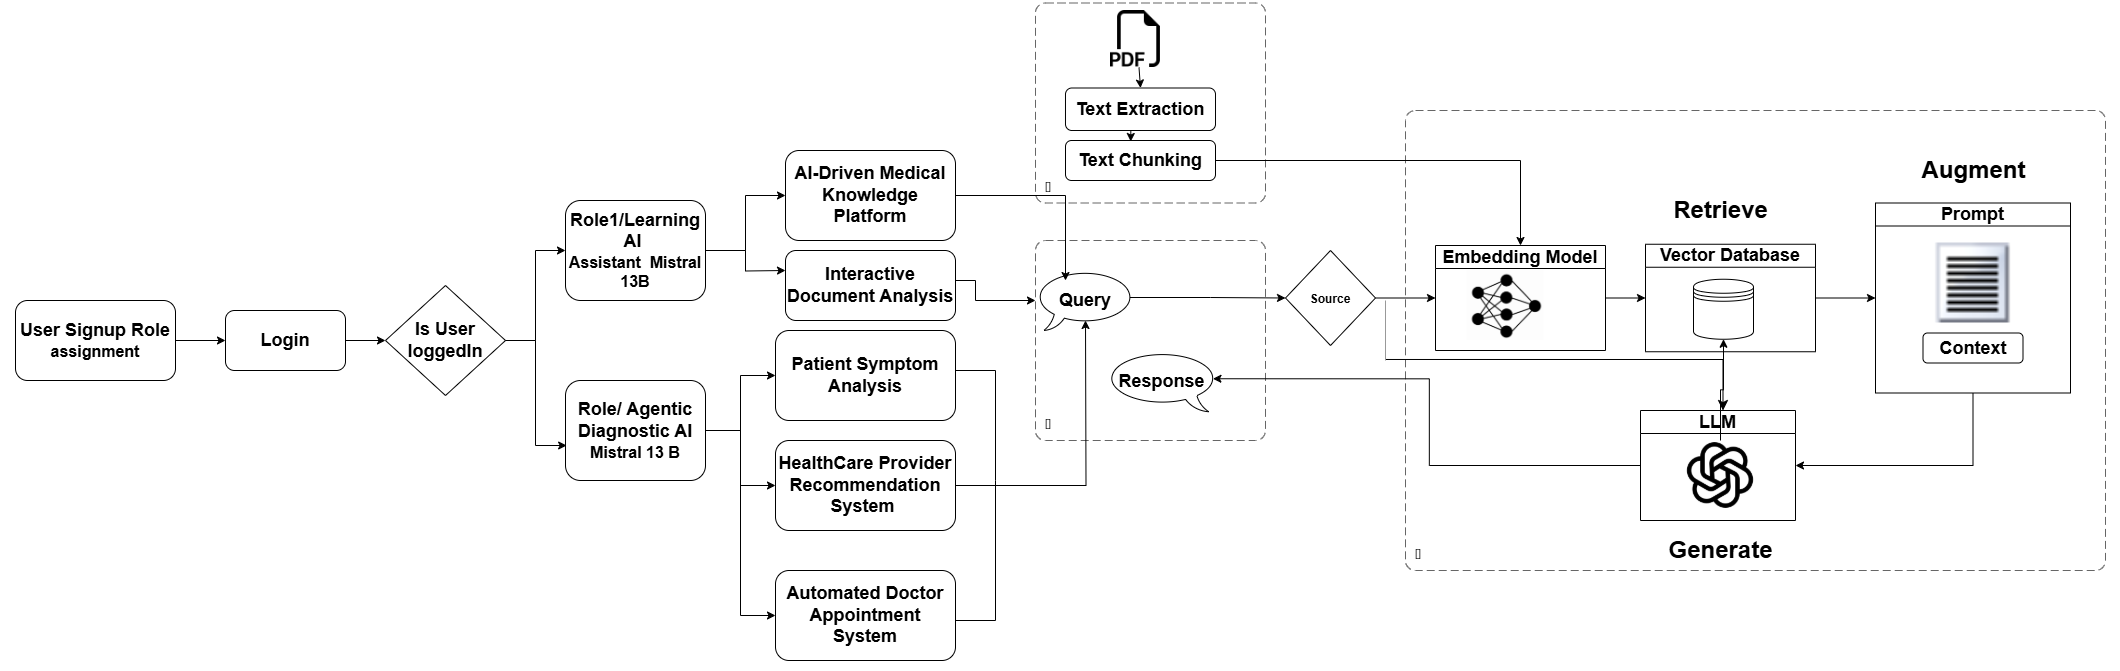
\includegraphics[width=15cm]{./Images/Thesis.png}
       \caption{Thesis implementation phases}
       \label{fig: Thesis implementation phases}
    \end{center}
    \end{figure}
% ============================================================================
% section : Data Collection and Analysis
% =============================================================================
\section{Data Collection and Analysis}

The data for this thesis is taken from the Fern Universität in Hagen, Germany. From the early 1980s to the present, 
Fern University has conducted numerous interviews as part of its contemporary history research projects. These include 
biographical interviews were individuals interviewees narrate their own stories and also gives their point of view on 
the events that occurred during that time. Apart from these biographical interviews, autobiographies, written texts and 
various letters are also collected from many people with different culture background but have a connection to social events 
in Germany. The video interviews are also present which has wide information about various topics like work councils, trade 
unionists, migrants, concentration camp survivors, and so on. The interviews contain some information
about the Germany history. There are about 350 Video interviews as part of the research which are convert into transcripts. 
The transcript of this dataset and contains three columns:

\begin{enumerate}
    \item\textbf{Timecode:} As the video interview is convert into transcript, the timecode is used to identify the 
    start and end of the interview. It is in the format of $hh:mm:ss$.
    \item\textbf{Sprecher:}  The name of the speaker in the interview.
    \item\textbf{Transcript:}  The interview transcript the conversation between the speakers.
\end{enumerate}
% ============================================================================
% section : Data Preprocessing
% =============================================================================
\section{Data Preprocessing}

Once the data is analysed it needs be Pre-processed in order to use it as the data might have mistaken, redundancies, 
missing values, or inconsistencies due to all these reasons it needs to be cleaned so that, we will be able to use it for 
further analysis. For example, during the training of a machine learning model it is important to clean the data in order 
to avoid overfitting or underfitting or wrong predictions. Hence, before using the dataset to any tasks it is better do some 
data cleaning if needed. There is not much Preprocessing is used in the thesis, but it is important to clean the data before 
using it. Few steps are followed in this thesis is mentioned below,

\begin{enumerate}
    \item\textbf{Removal of Unwanted columns}
    
    As the dataset has three columns of data, the timecode, the Sprecher and the transcript. In the Timecode column except 
    the timestamp of the video we don't have any information which can be used for analysis. Hence, it is removed.
    Sprecher column is removed as it is not required for the analysis. Since, it consists of the who speak that particular 
    sentence in the conversation and after analysis for the few transcripts it was not making much sense. Hence, it is removed.
    Transcript column is the key column which contains the main information of the conversation which is required for the analysis. 
    Here, the rows of the interviewer is not removed as may  contains the information which might be essential for the thesis.

    \item\textbf{Combining the data}
    
    As the dataset was in the excel format and each conversation transcript was in the form of a new line in the column 
    Transcript, it was necessary to combine the data into one single corpus. Hence, it is necessary to combine the data into 
    one a paragraph so that contexts of the conversation can be maintained, and which will help in the future phases. 
    On the other hand, the video conversation of each individual was available in the separate sheets in the excel file. 
    Hence, it is necessary to merge the data into a single text document. As the looping through each page and combining 
    them into a paragraph will take more time than the combination of the whole data. So, combining the data in one document
    will help to reduce the time taken for the analysis.

    \item\textbf{Removing the short sentences}
    
    As the transcript column was combined into a paragraph and there we have lot of sentences which are smaller than 3 words.
     This Sentence will act as nosie as there are repeated words, Stopwords, punctuations, etc. have formed the sentence which 
     is doesn't add value to the analysis as it is act like a noise in the data. Hence, it is necessary to remove all the sentences 
     that are smaller than 3 words. As it doesn't make sense to have a sentence with less than 3 words. So, filtered the short 
     sentences out of the dataset was done as it was like a noise in the data.

\end{enumerate}

There are few other steps that can be done to clean the data like Stopwords, punctuations, lemmatization, etc., which I haven't 
considered as it is not required. Since, these preprocessing is only required when we are doing word embedding hence, I have not 
considered it in the thesis. As I'll will doing sentence embedding which will help to capture the meaning of the sentences in 
the paragraph and get better results.
% ============================================================================
% section : Modelling
% =============================================================================


\section{Modelling}
In this stage, the approach of achieve topic modelling will be eaxplained. As the Preprocessing of the dataset is done. 
The dataset is ready for topic modelling where it will undergoes stages like embedding,
 dimensional reduction, clustering and generating the topic name using the language model. The various stages and mentioned 
 modelling techniques are explained by,
 \begin{figure}[htbp]
    \begin{center}
      \includegraphics[width=16cm]{./Images/Modelling Workflow.png}
       \caption{Modelling Workflow}
       \label{fig: Modelling Workflow}
    \end{center}
    \end{figure}
% ============================================================================
% subsection : Sentence Embedding
% =============================================================================
\subsection{Sentence Embedding}

After the Preprocessing of the dataset is done. The dataset is ready for embedding and as Sentence Embedding approach will 
be used to get the numerical representation of the text data which will help the machine learning model to understand the text data.
As the dataset is in German language choosing the good sentence embedding model is important to get better result as most of the 
embedding model are mostly trained on the English language Primary and then there are few models which are trained on multiple 
languages. So, choosing the good model is important to get better results. So, after careful examine some of the model for 
German language and few of the model is mentioned below,

 \begin{enumerate}
    \item GBERT Derived Embedding Models
    \item Sentence-T5 derived Models
    \item Paraphrase-multilingual
    \item Cross English \& German Roberta
    \item Jina embedding-v2-base-de
    \item German Sematic\_STS\_v2 and etc.,
\end{enumerate}

After comparing the models embedding and evaluating them, Jina embedding-v2-base-de and Cross English \& German Roberta model 
which work well in my scenario and by considering  all the other factors  like computational power, runtime, etc., 
I have chosen Jina embedding-v2-base-de model. As this model have a capabilities to handle both English and German text data 
along with it has been to work well in monolingual and cross-lingual applications without bias.

% ============================================================================
% subsection : Dimensionality Reduction
% =============================================================================

\subsection{Dimensionality Reduction}

The output of the embedding will be in very high dimensional space, and this cannot be used for further tasks. 
Therefore, in order to transform a high-dimensional vector space into a low-dimensional vector space, dimensionality
 reduction is necessary. There are lot of techniques that can be used for dimensionality reduction like PCA, t-SNE,
 UMAP, etc... For this thesis I have chosen UMAP reduction technique as it is a powerful and versatile dimensionality 
 reduction technique which has some of the advantages when compared to PCA (Principal Component Analysis), t-SNE 
 (t-distributed Stochastic Neighbour Embedding) and other techniques. Here is some of the reason why I have chosen 
 UMAP reduction technique,

\begin{enumerate}
    \item  It preserves the local and global structure of the data as it maintains the relationships between the data points
    at multiple scales, ensuring small groups and the global structure of the data is well represented at the reduced dimensional space.
    \item It is highly scalable and can be used for large datasets and its computational complexity is suitable for both small 
    and large sentence embeddings.
    \item One important aspect of sentence embedding is that it provides freedom in selecting the distance metric that is 
    used to determine the degree of similarity between the data points.
    \item It is faster and produces high quality embedding especially for large datasets when compared other technique.
    \item It will help to increase better cluster separation.
    \item This technique is quite versatile as it can be used for both dimensionality reduction and visualization.
\end{enumerate}

As UMAP, have lot of benefits like it is very scalable, efficient, flexible and can be used for large datasets and 
it doesn't consume much computational power when compared to other techniques.
This helps for producing meaningful results. 
% ============================================================================
% subsection : Clustering
% =============================================================================
\subsection{Clustering}

After the Dimensionality reduction is carried out for the embedding, the data is now ready for the clustering. In this phase, there are two cluster technique based on the scenario which can be used i.e., K-Means and HDBSCAN clustering.
By comparing the K-means and HDBSCAN clustering, I have chosen HDBSCAN as it is works well and has ability to cluster is well when compared to K-Means. Here are some of the reasons for choosing HDBSCAN over K-Means, 

\begin{enumerate}
    \item For K-Means Clustering, it is necessary to specify in advance how many clusters there are.
    \item It struggle we it tries to deal with the handling outliers.
    \item It tries to form uniform clusters of similar size as it assumes that all the clusters will be of same size.
\end{enumerate}

After looking into these aspects and choosing the HDBSCAN clustering, the technique works effectively for identifying the clusters of varying densities and robust to the noise which is suitable for our dataset. 
As HDBSCAN approach doesn't have a control on the creation of the clusters but, it can be configured with the help of parameters like minimum cluster size, minimum samples and dew other parameters which will help 
to form the clusters by considering the core point which ensures that the clustering process efficiently irrespective of data. By applying the HDBSCAN and UMAP technique, we will be able to uncover distinct clusters 
of semantically similar sentence to group them together and by filtering the noise and outliers. The formed clusters will be stored in the json format to feed the formed clusters to the Llama 3.1 model.
% ============================================================================
%  subsection : Language Model
% =============================================================================
\subsection{Language Model}
This is the final phase which will help to generate the topics for the given text. the clusters formed in the previous stage will be feed to Large Language model Llama 3.1. By providing the prompt along with the cluster, which will help 
the Language model to understand the sentences in the cluster and generate a generalized topic name for the particular clusters. This process involves leveraging the model’s ability to process and synthesize information from multiple 
sentences, producing a coherent and meaningful topic label for each cluster. The use of Llama 3.1 model ensures that the generated topic names are contextually appropriate and semantically meaningful, enhancing the interpretability
and utility of the cluster results. In this stage Llama 3.1 version model is used for the generation of topic names as it is the latest version open source model available and one of the powerful model which works efficiently 
for tasks like labelling, summarization, information retrieval, text generation and so on.

\section{Evaluation}
 The quality of the generated topics can be evaluated by comparing them with the human generated labels and by feeding the clusters to other open source large language model and models like LDA,
  NMF and BERTopic will give us a clarity of the quality of the generated topics. For evaluation of clustering, I have used Silhouette coefficient, davies bouldin score and calinski harabasz score.
  which will give the clear understanding of the quality of the clusters formed and also based on this we can identify how good the embedding model is. The metric helps to choose the right embedding
  model for the given dataset as embedding of text data is very important. If the embedding model is not well suited for the dataset, it will not be able to generate good clusters. So, with the help of
  Silhouette coefficient, davies bouldin score and calinski harabasz score we can understanding of the quality of the clusters formed  and how good the embedding has been done for the dataset.
  Along with this the topic generated by the Llama 3 model is compared with the human estimation so that, we can understand the quality of the topics generated and by feeding the clusters to other
  open source large language model which will give us a clarity of the quality of the generated topics. With the help of these metrics, I have compared the clusters formed and the generated topics of the model with human estimation.

% ============================================================================
% section : Summary
% =============================================================================
\section{Summary}

This chapter was about the explanation of step-by-step process which was followed to accomplish this thesis. Starting from data collection where data was understood and analysed to know the structure of the data then,
 preprocessing of the data were unwanted columns and noise were eliminated and combined into a single paragraph was done. After that, the data was converted into numerical representation using the embedding technique 
 followed by dimensionality reduction and clustering.



\chapter{Implementation}

\label{Chapter4}
In this chapter, a comprehensive overview of the libraries utilized throughout the project is presented, 
alongside the roles each library plays in different sections of the code. By offering deeper insight 
into how each component works and how the algorithms are implemented, this thesis is brought to its conclusion.

For the implementation of the thesis, I have used platforms such as VS Code (Visual Studio Code) and Jupyter Notebook. 
While VS Code is an integrated development environment (IDE) suitable for a variety of languages and extensions, 
Jupyter Notebook offers a web-based environment that is well-suited for interactive coding and data visualization.


\vspace{1cm}
%%%%%%%%%%%%%%%%%%%%%%%%%%%%%%%%%%%%%%%%
\section{Libraries}
%%%%%%%%%%%%%%%%%%%%%%%%%%%%%%%%%%%%%%%%
In this section, we focus on the various libraries used in the project and how they contribute to the overall model implementation process.

\vspace{0.4cm}
%%%%%%%%%% sqlite3 %%%%%%%%%%
\noindent\textbf{sqlite3:}

\noindent
The \texttt{sqlite3} module is part of Python’s standard library, enabling lightweight database operations. 
It is used here to store and retrieve user information, roles, and session data. This is particularly helpful 
for managing authentication details in a local, file-based database, without requiring an external database server \cite{sqlite3}.

\vspace{0.4cm}
%%%%%%%%%% httpcore %%%%%%%%%%
\noindent\textbf{httpcore (TimeoutException):}

\noindent
\texttt{httpcore} is a low-level HTTP library used to manage connection pooling, timeouts, and retries. 
In this thesis, it is mainly leveraged to handle \texttt{TimeoutException} cases, ensuring the application 
does not hang indefinitely during network calls \cite{httpcore}.

\vspace{0.4cm}
%%%%%%%%%% Selenium %%%%%%%%%%
\noindent\textbf{Selenium:}

\noindent
Selenium automates browsers, enabling dynamic web scraping. It is used in conjunction with the Edge WebDriver
to navigate pages, locate elements, and extract data. Relevant classes such as \texttt{Service}, \texttt{Options}, 
and \texttt{WebDriverWait} help in configuring and controlling the browser for scraping tasks \cite{selenium}.

\vspace{0.4cm}
%%%%%%%%%% BeautifulSoup %%%%%%%%%%
\noindent\textbf{BeautifulSoup (bs4):}

\noindent
\texttt{BeautifulSoup} parses HTML (and XML) content, transforming the raw webpage data into a navigable tree. 
Used together with Selenium, it allows the program to extract specific tags, links, or other structured elements 
from the loaded pages \cite{beautifulsoup}.

\vspace{0.4cm}
%%%%%%%%%% time %%%%%%%%%%
\noindent\textbf{time:}

\noindent
This built-in Python module provides sleep intervals and basic time management. Incorporating small delays can prevent 
overwhelming target servers, especially when performing repetitive automated scraping \cite{time}.

\vspace{0.4cm}
%%%%%%%%%% json %%%%%%%%%%
\noindent\textbf{json:}

\noindent
The \texttt{json} module encodes and decodes data in JSON (JavaScript Object Notation). It is both human-readable
and language-independent, making it ideal for transmitting and storing structured data. In this project, JSON 
formats are used to manage intermediate results, user sessions, or to pass data between components \cite{json}.

\vspace{0.4cm}
%%%%%%%%%% chainlit %%%%%%%%%%
\noindent\textbf{chainlit:}

\noindent
\texttt{chainlit} provides a framework for building chat-based interfaces around large language models (LLMs). 
It handles session management, real-time conversation flows, and prompt configuration, giving users an 
intuitive platform to interact with AI-driven functionalities \cite{chainlit}.

\vspace{0.4cm}
%%%%%%%%%% src.helper (download_hugging_face_embeddings) %%%%%%%%%%
\noindent\textbf{src.helper:}

\noindent
While not a standard library, this local module contains custom utilities such as \texttt{download\_hugging\_face\_embeddings}. 
It automates loading the required embeddings from Hugging Face, ensuring consistent embedding generation 
across the system \cite{pinecone}.

\vspace{0.4cm}
%%%%%%%%%% langchain_community.vectorstores (Pinecone) %%%%%%%%%%
\noindent\textbf{langchain\_community.vectorstores (Pinecone):}

\noindent
This integration connects LangChain’s data processing workflows with the Pinecone vector database. By creating embeddings 
and storing them in Pinecone, the system retrieves similar text chunks or documents quickly, enhancing response accuracy 
in the chatbot \cite{langchain}.

\vspace{0.4cm}
%%%%%%%%%% pinecone (PineconeClient, ServerlessSpec) %%%%%%%%%%
\noindent\textbf{pinecone:}

\noindent
The \texttt{pinecone} SDK communicates with the Pinecone service, a specialized vector database built for high-speed 
similarity search. \texttt{PineconeClient} handles index creation and queries, while \texttt{ServerlessSpec} configures 
the underlying infrastructure \cite{pinecone}.

\vspace{0.4cm}
%%%%%%%%%% langchain.prompts (PromptTemplate) %%%%%%%%%%
\noindent\textbf{langchain.prompts (PromptTemplate):}

\noindent
\texttt{PromptTemplate} structures how queries are fed into large language models. By separating static and dynamic 
parts of a prompt, it creates systematic instructions for LLM-based generation \cite{langchain}.

\vspace{0.4cm}
%%%%%%%%%% langchain_community.llms (CTransformers) %%%%%%%%%%
\noindent\textbf{langchain\_community.llms (CTransformers):}

\noindent
\texttt{CTransformers} provides an interface for loading and running transformer models within the LangChain ecosystem. 
It can be more memory-efficient and can help speed up inference in certain configurations \cite{sentence_transformers}.

\vspace{0.4cm}
%%%%%%%%%% langchain.chains (RetrievalQA) %%%%%%%%%%
\noindent\textbf{langchain.chains (RetrievalQA):}

\noindent
\texttt{RetrievalQA} coordinates the search of relevant vectors/documents before the final language model call. 
This leads to more accurate, context-specific responses to user questions, making the chatbot more robust \cite{langchain}.

\vspace{0.4cm}
%%%%%%%%%% langchain.document_loaders (PyPDFLoader) %%%%%%%%%%
\noindent\textbf{langchain.document\_loaders (PyPDFLoader):}

\noindent
\texttt{PyPDFLoader} helps parse PDF documents into text chunks, enabling easy ingestion of content into the retrieval 
system. This is crucial when dealing with PDF-based data sets \cite{langchain}.

\vspace{0.4cm}
%%%%%%%%%% langchain.text_splitter (CharacterTextSplitter) %%%%%%%%%%
\noindent\textbf{langchain.text\_splitter (CharacterTextSplitter):}

\noindent
Splits text into manageable chunks based on character count. By doing so, the system can embed and retrieve smaller, 
more relevant pieces of information during user queries \cite{langchain}.

\vspace{0.4cm}
%%%%%%%%%% dotenv (load_dotenv) %%%%%%%%%%
\noindent\textbf{dotenv (load\_dotenv):}

\noindent
Loads environment variables from a \texttt{.env} file, preventing sensitive credentials (like API keys) from 
being exposed in the source code. This approach enhances security and deployment flexibility \cite{dotenv}.

\vspace{0.4cm}
%%%%%%%%%% sentence_transformers (SentenceTransformer) %%%%%%%%%%
\noindent\textbf{sentence\_transformers:}

\noindent
This library provides state-of-the-art models for sentence and paragraph embeddings. By embedding text into vector 
representations, the system can compare semantic similarities and rank documents according to relevance \cite{sentence_transformers}.

\vspace{0.4cm}
%%%%%%%%%% twilio.rest (Client) %%%%%%%%%%
\noindent\textbf{twilio.rest (Client):}

\noindent
Twilio’s Python SDK handles sending SMS messages or other communications. The chatbot uses this to send appointment 
reminders or booking confirmations to users, enhancing the system’s real-world utility \cite{sentence_transformers}.

\vspace{0.4cm}
%%%%%%%%%% os %%%%%%%%%%
\noindent\textbf{os:}

\noindent
A built-in Python module for OS-level interactions, such as file path handling and environment variable lookups. 
Used to coordinate local file structure and manage \texttt{.env} variables \cite{os}.

\vspace{0.4cm}
%%%%%%%%%% logging %%%%%%%%%%
\noindent\textbf{logging:}

\noindent
\texttt{logging} is the standard Python library for capturing and recording logs, warnings, and error messages. 
It helps in debugging and monitoring the application’s performance \cite{logging}.

\vspace{0.4cm}
%%%%%%%%%% warnings %%%%%%%%%%
\noindent\textbf{warnings:}

\noindent
The \texttt{warnings} module is used to handle non-critical warnings in Python. In this context, it can hide or filter 
out messages from dependencies that are not relevant to the end-user \cite{warnings}.

\vspace{0.4cm}
%%%%%%%%%% asyncio %%%%%%%%%%
\noindent\textbf{asyncio:}

\noindent
\texttt{asyncio} facilitates concurrent execution of tasks, leveraging an event loop to handle long-running or 
I/O-bound processes without blocking other functionalities. Particularly useful for background tasks in chatbots \cite{pythonlibrary}.

\vspace{0.4cm}
%%%%%%%%%% flask %%%%%%%%%%
\noindent\textbf{Flask:}

\noindent
Flask is a lightweight Python framework used to build web applications and RESTful APIs. 
It manages server-side processes, routes, and user sessions, playing an important role in bridging
the front-end user interface with back-end logic \cite{flask}.

\vspace{0.4cm}
%%%%%%%%%% database (init_db, get_user, add_user) %%%%%%%%%%
\noindent\textbf{database:}

\noindent
This local Python module contains functions like \texttt{init\_db}, \texttt{get\_user}, and \texttt{add\_user}, 
supporting user registration, retrieval, and management. It leverages \texttt{sqlite3} to store and fetch user credentials.

\vspace{0.4cm}
%%%%%%%%%% subprocess %%%%%%%%%%
\noindent\textbf{subprocess:}

\noindent
The \texttt{subprocess} module lets you spawn new processes, connect to their input/output/error pipes,
and obtain their return codes. This functionality is essential when starting or stopping auxiliary services 
like a Chainlit server \cite{subprocess}.

\vspace{0.4cm}
%%%%%%%%%% threading %%%%%%%%%%
\noindent\textbf{threading:}

\noindent
\texttt{threading} supports concurrency by running multiple threads in parallel. In this project, it helps 
avoid blocking the main application by delegating tasks (such as server checks) to background threads \cite{threading}.

\vspace{0.4cm}
%%%%%%%%%% requests %%%%%%%%%%
\noindent\textbf{requests:}

\noindent
\texttt{requests} simplifies making HTTP requests. It is used to communicate with external APIs (e.g., Pinecone, 
Twilio, or third-party services) and verify that local services like Chainlit are up and running \cite{requests}.

\vspace{0.4cm}
%%%%%%%%%% numpy %%%%%%%%%%
\noindent\textbf{numpy:}

\noindent
\texttt{numpy} provides a multi-dimensional array object and routines for fast array manipulations, 
serving as the fundamental package for numerical computations in Python \cite{numpy}.


\vspace{1cm}
\noindent\textbf{HTML/CSS:}

The front-end user interface is structured using HTML and styled with CSS. HTML forms gather user input, 
while CSS ensures the layout is visually appealing and user-friendly. This combo supports usability 
and meets the requirements for practical deployment.

%%%%%%%%%% Code Implementation %%%%%%%%%%%

\section{Code Implementation}

In this chapter, we map the major steps of our architecture (see Figure~\ref{fig:system-architecture}) to their respective code components. Each section follows the flow of data and logic from user authentication all the way to generating a final answer.

\section{User Authentication and Role Identification}
\label{sec:auth-role}
User management begins with:
\begin{itemize}
    \item \textbf{Signup \& Role Assignment:} A new user provides an email and password. The system assigns the role (\textit{e.g., patient} or \textit{medical student}) by storing it in a lightweight database (e.g., using \texttt{sqlite3}).
    \item \textbf{Login:} On login, the code checks the role from the database to serve the correct chatbot mode.
    \item \textbf{Session Handling:} Flask or Chainlit stores session data (e.g., user email and role) so each request can correctly route to patient or student logic.
\end{itemize}

\section{PDF Processing (Text Extraction and Chunking)}
\label{sec:pdf-chunking}
PDF documents (e.g., medical articles) are uploaded by students:
\begin{itemize}
    \item \textbf{Extraction:} The code typically uses a library like \texttt{PyPDFLoader} to read and convert PDF pages to raw text.
    \item \textbf{Chunking:} Long text is split into manageable pieces via \texttt{CharacterTextSplitter} or custom splitting logic, ensuring each chunk remains semantically coherent. 
    \item \textbf{Preprocessing:} Code may further remove stopwords or apply cleaning to each chunk before embedding.
\end{itemize}

\section{Embedding Generation}
\label{sec:embedding}
Each text chunk is converted into a numerical representation (an \textit{embedding}):
\begin{itemize}
    \item \textbf{Model Setup:} A pretrained model (e.g., \texttt{all-mpnet-base-v2} or \texttt{SentenceTransformer}) is loaded.
    \item \textbf{Batch Embedding:} The code loops through chunks and feeds them into the embedding model. This step often includes concurrency or batch processing to optimize runtime.
    \item \textbf{Storage:} Embeddings are passed either to an in-memory structure or a vector database (such as Pinecone) for fast retrieval.
\end{itemize}

\section{Pinecone Vector Database}
\label{sec:pinecone}

After the system generates embeddings for each text chunk (Section~\ref{sec:embedding}), the next step is to store them in a vector database for fast retrieval. Here, we integrate with \emph{Pinecone} to manage and query these embeddings efficiently:

\begin{itemize}
    \item \textbf{Index Creation}: The system checks whether an index (e.g., \texttt{"zf"}) already exists in Pinecone. If not, it creates one with a specified dimension (e.g., 768) and metric (e.g., \texttt{cosine}). This ensures compatibility with the selected embedding model (e.g., \texttt{all-mpnet-base-v2}).
    \item \textbf{Batch Upload}: Each text chunk is embedded (transformed into a numerical vector) and then stored in Pinecone with a unique identifier. Doing so in batches reduces overhead when dealing with large datasets.
    \item \textbf{High-Speed Retrieval}: When the user asks a question or enters a search query, the system converts their text into an embedding and performs a similarity search against the Pinecone index. The top-$k$ most relevant chunks are returned to provide context for LLM-based responses (Section~\ref{sec:rag-pipeline}).
    \item \textbf{Scalability \& Flexibility}: Pinecone accommodates millions of embeddings and quickly returns nearest neighbors, allowing the system to handle ever-growing corpora of PDF documents, scraped data, or other text sources without re-processing older content.
\end{itemize}

By coupling embeddings (Section~\ref{sec:embedding}) with Pinecone’s vector database, the system can efficiently surface contextual insights and pass them to the Large Language Model for retrieval-augmented generation. This approach significantly boosts the accuracy and relevance of chatbot answers, particularly in a medical or academic setting where precise factual references are paramount.


\section{Retrieval-Augmented Generation Pipeline}
\label{sec:rag-pipeline}
To handle user queries, we blend retrieval (based on embeddings) with LLM generation:
\begin{itemize}
    \item \textbf{Query Handling:} Once a user query arrives, the system transforms it into an embedding (using the same model as above).
    \item \textbf{Similarity Search:} This embedding is compared against stored embeddings in Pinecone (or another vector store). The top-$k$ relevant chunks are returned.
    \item \textbf{Prompt Augmentation:} These chunks are appended to the user’s query to form a “context window” for the Large Language Model (LLM).
    \item \textbf{Response Generation:} The LLM (e.g., Mistral 13B) produces an answer grounded in the retrieved text. The code also applies any prompt template rules or role-specific instructions.
\end{itemize}

\section{Role-Based Logic (Learning Assistant vs. Diagnostic Agent)}
\label{sec:role-logic}
In the code, a conditional block or chain-level branching typically handles:
\begin{itemize}
    \item \textbf{Student Mode (Learning AI Assistant)}:  
    Provides detailed, in-depth explanations with references.
    \item \textbf{Patient Mode (Agentic Diagnostic AI)}:  
    Focuses on simpler language, symptom triage, or booking logic. 
    When users mention booking an appointment, an agentic step can automatically interact with a scheduling API.
\end{itemize}

\section{Symptom Analysis, Provider Recommendation, and Appointment Booking}
\label{sec:extended-capabilities}



For patient-focused tasks, code sections may:
\begin{itemize}
    \item \textbf{Symptom Analysis}: Use a rule-based approach or LLM prompts fine-tuned on medical data to interpret user symptoms.
    \item \textbf{Provider Recommendation}: Parse a local database (or external service) of doctors. The code filters by specialty or location, returning suitable recommendations.
    \item \textbf{Appointment Booking}: Integrate with an external API (e.g., Twilio for SMS, Doctolib for scheduling). The code triggers a request, confirms details, and notifies the user.
\end{itemize}

\section{Front-End }
\label{sec:frontend}
\begin{itemize}
    \item \textbf{Flask or Chainlit Routes}: A Python route handles file uploads (for PDFs) or query input. These routes pass data to the back-end logic (embedding, retrieval, LLM).
    \item \textbf{User Interface}: HTML/CSS or a Chainlit-based chat bubble interface. The code updates the chat context in real-time and displays responses from the LLM.
    \item \textbf{Templating}: If using Flask, Jinja templates might render dynamic pages with user-specific data.
\end{itemize}

\section{Error Handling and Logging}
\label{sec:error-logging}
Throughout the system:
\begin{itemize}
    \item \textbf{Try-Except Blocks}: Key places (e.g., PDF loading, retrieval queries, LLM calls) are wrapped in \texttt{try-except} to gracefully handle failures.
    \item \textbf{Logging}: The Python \texttt{logging} module or a custom logger records warnings, debug info, and errors. This helps in diagnosing issues without exposing them to end users.
    \item \textbf{Notifications}: In critical scenarios (like an inability to retrieve from the vector database), the code might send an alert or fallback to a simpler pipeline.
\end{itemize}

\section{User Authentication and Role Identification Integration}
\label{sec:auth-role}

Below is an excerpt of Python/Flask code illustrating how user login, signup, and role identification are handled:

\begin{lstlisting}[language=Python, caption={User authentication and role assignment code}, basicstyle=\small\ttfamily]
from flask import Flask, render_template, request, redirect, url_for
from database import init_db, get_user, add_user
import subprocess
import threading
import os
import time
import requests

app = Flask(__name__)

# Initialize the database
init_db()

FLASK_PORT = 5002
CHATBOT_PORT = 8001
chainlit_process = None

def is_chainlit_running():
    try:
        response = requests.get(f"http://localhost:{CHATBOT_PORT}")
        return response.status_code == 200
    except requests.exceptions.ConnectionError:
        return False

def start_chainlit(email):
    global chainlit_process
    if is_chainlit_running():
        print("Chainlit is already running.")
        return

    print(f"Launching Chainlit on port {CHATBOT_PORT}...")
    chainlit_process = subprocess.Popen(
        ["chainlit", "run", "app.py", "--port", str(CHATBOT_PORT)],
        cwd=os.path.dirname(os.path.abspath(__file__)),
        stdout=subprocess.DEVNULL,
        stderr=subprocess.DEVNULL,
        start_new_session=True,
        env={
            os.environ,
            "LOGGED_IN_EMAIL": email
        }
    )

@app.route("/", methods=["GET", "POST"])
def login():
    """Login route to authenticate users and start Chainlit."""
    if request.method == "POST":
        email = request.form.get("email")
        password = request.form.get("password")
        user = get_user(email)
        if user and user[2] == password:
            print(f"LOGIN SUCCESS: {email}")

            # Start Chainlit if not running; pass the email to the new process
            threading.Thread(target=start_chainlit, args=(email,), daemon=True).start()

            # After login, display a loading page that will link to Chainlit
            chatbot_url = f"http://localhost:{CHATBOT_PORT}/"
            print(f"REDIRECTING TO: {chatbot_url}")
            return render_template("loading.html", chatbot_url=chatbot_url)
        else:
            return render_template("login.html", error="Invalid email or password.")
    return render_template("login.html")

@app.route("/signup", methods=["GET", "POST"])
def signup():
    """Signup route to register new users."""
    if request.method == "POST":
        email = request.form.get("email")
        password = request.form.get("password")
        role = request.form.get("role")
        if add_user(email, password, role):
            return redirect(url_for("login"))
        else:
            return render_template("signup.html", error="Email already registered.")
    return render_template("signup.html")

if __name__ == "__main__":
    app.run(port=FLASK_PORT, debug=True)
\end{lstlisting}

\subsection{Initialization of the Database}
\begin{itemize}
  \item \texttt{init\_db()}: Called immediately upon starting the Flask application to ensure that the local SQLite
        database (or whichever database is being used) is properly initialized. This might create tables such as
        \texttt{users} if they do not exist.
\end{itemize}

\subsection{Signup Logic}
\label{subsec:signup}
\begin{itemize}
  \item \textbf{Route:} \texttt{/signup} handles both \texttt{GET} (displaying a signup form) and \texttt{POST} (processing form data).
  \item \textbf{Form Inputs:} Users provide \texttt{email}, \texttt{password}, and \texttt{role} (for example, ``PATIENT'' or ``STUDENT'').
  \item \textbf{add\_user}: A database function that inserts a new record into the \texttt{users} table. If the operation
        is successful, the user is redirected to the login page; otherwise, an error is displayed
        (e.g. ``Email already registered'').
\end{itemize}

\subsection{Login Logic}
\label{subsec:login}
\begin{itemize}
  \item \textbf{Route:} \texttt{/} or \texttt{/login}, handling both \texttt{GET} (showing the login template) and
        \texttt{POST} (verifying credentials).
  \item \textbf{Credential Check:} The user’s provided email is passed to \texttt{get\_user(email)}, which queries the
        database for a matching record (typically returning a tuple \((id, email, password, role)\)).
  \item \textbf{Password Match:} \texttt{user[2] == password} ensures the stored password matches the user’s input.
        If it matches, login is considered successful.
  \item \textbf{Chainlit Process:} After a successful login, the function \texttt{start\_chainlit(email)} is triggered
        in a background thread. This:
        \begin{enumerate}
            \item Checks if Chainlit is already running via \texttt{is\_chainlit\_running()}.
            \item If not running, spawns a subprocess with the user’s email set as an environment variable. This email
                  can then be used by the chatbot to fetch the user’s role from the database without needing URL parameters.
        \end{enumerate}
  \item \textbf{Redirect to Loading Screen:} 
        \begin{itemize}
          \item Renders the template \texttt{loading.html}, which contains a link or auto-redirect to the running Chainlit instance at \texttt{http://localhost:8001}.
        \end{itemize}
  \item \textbf{Error Handling:} If the email/password is incorrect, the user is shown the \texttt{login.html} form
        again, this time with an error message (``Invalid email or password'').
\end{itemize}

\subsection{Role Identification \& Usage}
\begin{itemize}
  \item \textbf{During Signup:} 
  \begin{enumerate}
    \item The \texttt{role} field is selected by the user or assigned automatically (e.g., \texttt{PATIENT} or \texttt{STUDENT}).
    \item \texttt{add\_user} stores the role in the database alongside the \texttt{email} and \texttt{password}.
  \end{enumerate}
  \item \textbf{During Login:}
  \begin{enumerate}
    \item Once the login is validated, the user’s \texttt{role} can be fetched from \texttt{user[3]}. 
    \item In a fully built system, the chatbot interface might reference this role to load different conversation chains
          or specialized functionality. For instance:
          \begin{itemize}
            \item \emph{Medical Students} might get an LLM chain focusing on advanced medical knowledge.
            \item \emph{Patients} might see simplified symptom analysis tools and appointment booking flows.
          \end{itemize}
  \end{enumerate}
\end{itemize}

\subsection{Chainlit Integration}
\label{subsec:chainlit}
\begin{itemize}
  \item \textbf{is\_chainlit\_running()}: Sends an HTTP GET request to \texttt{http://localhost:8001} (the configured Chainlit port).
        If the server responds with a \texttt{200} status code, we assume Chainlit is active.
  \item \textbf{start\_chainlit(email)}: 
        \begin{enumerate}
            \item Uses \texttt{subprocess.Popen} to run \texttt{chainlit} on the given port if not already running.
            \item Exports \texttt{LOGGED\_IN\_EMAIL} as an environment variable. 
                  This allows the Chainlit app to retrieve the user’s role from the database with the same email,
                  applying role-specific logic during chatbot interactions.
        \end{enumerate}
\end{itemize}

\subsection{Overall Flow}
\begin{enumerate}
  \item A new user signs up using \texttt{/signup}, providing email, password, and role.
  \item The system calls \texttt{add\_user} to store these details in the local database.
  \item The user then goes to \texttt{/login}, enters the same email and password, which \texttt{get\_user} verifies.
  \item If successful, \texttt{start\_chainlit} is triggered, launching or reusing a Chainlit session for the user.
  \item The user is redirected to a loading page and then to the Chainlit UI, where their role (retrieved from the database) 
        dictates the AI chatbot’s behavior.
\end{enumerate}

\noindent
In short, this code section ensures:
\begin{itemize}
    \item Secure handling of login and signup flows.
    \item Automatic role assignment and retrieval from the database.
    \item Seamless bridging between the Flask web server and the Chainlit chatbot interface.
\end{itemize}

\section{PDF Processing (Text Extraction and Chunking) Integration}
\label{sec:pdf-chunking}

In this part of the code, we handle the user-uploaded PDF files—from reading the file’s pages to splitting the text into smaller segments (chunks) that are later added to our vector store for retrieval. Below is a detailed snippet and explanation:

\begin{lstlisting}[language=Python, caption={PDF Processing and Chunking}, basicstyle=\small\ttfamily]
# If user uploaded a file via paperclip
if message.type == "file":
    logging.info("Processing uploaded file from user via paperclip...")

    # 1 Load the PDF using PyPDFLoader
    loader = PyPDFLoader(message.file_path)
    documents = loader.load()

    # 2 Split text into smaller chunks
    text_splitter = CharacterTextSplitter(chunk_size=4000, chunk_overlap=500)
    texts = text_splitter.split_documents(documents)

    # 3 Add the chunks to the vector store in manageable batches
    batch_size = 10
    for i in range(0, len(texts), batch_size):
        batch = [t.page_content for t in texts[i : i + batch_size]]
        docsearch.add_texts(batch)

    # 4 Notify the user about successful processing
    await cl.Message(
        content=(
            "PDF uploaded and processed successfully! "
            "You can now ask questions about its content."
        )
    ).send()

    return
\end{lstlisting}

\subsubsection*{Detailed Explanation}

\begin{enumerate}
    \item \textbf{Detecting a File Upload}
    \begin{itemize}
        \item The code checks if \texttt{message.type == "file"}. If so, it logs a message indicating that a PDF file has been received from the user through the paperclip icon in Chainlit.
        \item Using an \texttt{if} condition around the file-logic ensures text messages and file uploads are handled separately in the same event function.
    \end{itemize}

    \item \textbf{Loading the PDF with \texttt{PyPDFLoader}}
    \begin{itemize}
        \item \texttt{PyPDFLoader} is a document loader that reads PDF files and converts them into a list of \texttt{Document} objects—one for each page. 
        \item Internally, it might use a library like PyPDF2 or pdfplumber to extract text. Here, \texttt{loader.load()} creates an in-memory representation of the PDF content as \texttt{documents}.
    \end{itemize}

    \item \textbf{Splitting Text into Chunks}
    \begin{itemize}
        \item Why split? Large text blocks can overwhelm certain embedding or retrieval systems. Breaking down pages into chunks helps keep context manageable and supports more accurate retrieval results (since each chunk remains more focused on a single topic).
        \item \texttt{CharacterTextSplitter}:
        \begin{itemize}
          \item \texttt{chunk\_size=4000} sets the maximum number of characters in a chunk.
          \item \texttt{chunk\_overlap=500} ensures a 500-character overlap between consecutive chunks. This overlap helps preserve continuity of context between two consecutive chunks. When retrieving answers, slightly overlapping text can prevent abrupt context cuts.
        \end{itemize}
        \item \texttt{text\_splitter.split\_documents(documents)}:
        \begin{itemize}
            \item Loops over each \texttt{Document} (e.g., each PDF page) and subdivides it into multiple, partially-overlapping text segments.
            \item Returns a list of \textit{split} text segments, stored in the \texttt{texts} variable. 
        \end{itemize}
    \end{itemize}

    \item \textbf{Batch Insertion into the Vector Store}
    \begin{itemize}
        \item A \textit{vector store} (like Pinecone) is used to store embeddings so that relevant chunks can be quickly retrieved based on semantic similarity.
        \item We define \texttt{batch\_size = 10} to avoid feeding all chunks at once, which could be memory-intensive if the PDF is large.
        \item The loop \texttt{for i in range(0, len(texts), batch\_size)} processes chunks in increments of 10. Each iteration:
        \begin{enumerate}
            \item Slices a \texttt{batch} of 10 from the \texttt{texts} list.
            \item Calls \texttt{docsearch.add\_texts(batch)} to add that subset of chunks to the vector database. 
        \end{enumerate}
        \item Splitting into batches ensures stable performance and reduces the risk of timeouts or memory spikes.
    \end{itemize}

    \item \textbf{User Notification}
    \begin{itemize}
        \item After successfully uploading and splitting the PDF content, the user is informed with a message (``PDF uploaded and processed successfully!''). 
        \item This immediate feedback ensures a good user experience by confirming that the system is ready to handle queries about the newly indexed content.
    \end{itemize}

    \item \textbf{Return Statement}
    \begin{itemize}
        \item The function ends (\texttt{return}) to avoid further processing of the \texttt{message} as if it were a text query. 
        \item This prevents any additional or conflicting logic from executing once the file-handling code finishes.
    \end{itemize}
\end{enumerate}

\subsubsection*{Why Chunking is Important}
\begin{itemize}
  \item \textbf{Efficient Retrieval:} Many LLM-based retrieval systems do best when dealing with smaller segments. Searching and re-ranking short chunks is often faster and more precise.
  \item \textbf{Context Preservation:} Overlapping chunks maintain local context across boundary areas, which is crucial for question answering. If text relevant to a user’s question is split between the end of one chunk and the start of the next, the chunk overlap ensures minimal information loss.
  \item \textbf{Scalability:} Large PDF files with dozens or even hundreds of pages become more manageable. The user can ask questions about any part of the document without manually referencing page numbers or paragraphs.
\end{itemize}

This upload, split, and index workflow is central to enabling a dynamic question-answer system, where each user can bring in new documents and instantly query them. Once the text is converted into vector form, the system can retrieve it for any subsequent queries, seamlessly integrating new medical or academic documents into the user’s knowledge base.

\section{Embedding Generation Integration}
\label{sec:embedding-generation}

This portion of the code lays out how we prepare a sentence-level embedding model and connect it to the vector database—ensuring that new text segments are converted into numerical vectors (embeddings). Below is the relevant snippet, with an in-depth discussion:

\begin{lstlisting}[language=Python, caption={Embedding Model Setup and Pinecone Integration}, basicstyle=\small\ttfamily]
# 1 Load embeddings for all-mpnet-base-v2 (768-dimensional embeddings)
embedding_model = SentenceTransformer('all-mpnet-base-v2')
embeddings = download_hugging_face_embeddings()

# 2 Initialize Pinecone
pinecone_instance = PineconeClient(api_key=PINECONE_API_KEY)
if index_name not in [index.name for index in pinecone_instance.list_indexes()]:
    pinecone_instance.create_index(
        name=index_name,
        dimension=768,
        metric='cosine',
        spec=ServerlessSpec(cloud='aws', region=PINECONE_API_ENV)
    )

# 3 Access the index
docsearch = Pinecone.from_existing_index(index_name, embeddings)
\end{lstlisting}

\subsubsection*{Step-by-Step Explanation}
\begin{enumerate}
    \item \textbf{Loading the Embedding Model}
    \begin{itemize}
        \item \texttt{SentenceTransformer(\textquotesingle all-mpnet-base-v2\textquotesingle)}: 
        We instantiate a pre-trained embedding model from the \emph{Sentence Transformers} family.  
        \begin{itemize}
            \item \emph{all-mpnet-base-v2} outputs vectors of size 768 for each sentence or text chunk.
            \item This particular model is well-regarded for capturing semantic similarities, making it suitable for question answering or retrieval tasks.
        \end{itemize}

        \item \texttt{embeddings = download\_hugging\_face\_embeddings()}: 
        A custom utility, presumably in \texttt{src.helper}, that either fetches or caches embedding-related data.  
        \begin{itemize}
            \item This may ensure version consistency, or optimize performance by not repeatedly downloading large model files.
            \item The result is likely a reference to the same dimension/embedding pipeline used by \texttt{SentenceTransformer}, meaning the code can embed both documents and user queries in a matching format.
        \end{itemize}
    \end{itemize}

    \item \textbf{Initializing Pinecone (Vector Database)}
    \begin{itemize}
        \item \texttt{pinecone\_instance = PineconeClient(api\_key=PINECONE\_API\_KEY)}: 
        This sets up communication with Pinecone’s vector database, using the API key provided via environment variables.
        \item We then check whether our target \texttt{index\_name} (here, \texttt{zf}) exists:
        \begin{itemize}
            \item \texttt{pinecone\_instance.list\_indexes()} returns a list of existing indexes.
            \item If \texttt{zf} is missing, we call \texttt{pinecone\_instance.create\_index(...)}:
            \begin{itemize}
                \item \texttt{dimension=768} aligns with the output dimension of \texttt{all-mpnet-base-v2}.
                \item \texttt{metric='cosine'} ensures we measure distance (or similarity) in terms of cosine similarity, which is a common choice for text embeddings.
                \item \texttt{ServerlessSpec} configures the environment (e.g., \texttt{cloud='aws'}, \texttt{region=PINECONE\_API\_ENV}), controlling where the index is hosted.
            \end{itemize}
        \end{itemize}
        \item If an index called \texttt{zf} already exists, creation is skipped—this prevents overwriting data.
    \end{itemize}

    \item \textbf{Linking the Embedding Model to the Index}
    \begin{itemize}
        \item \texttt{docsearch = Pinecone.from\_existing\_index(index\_name, embeddings)}: 
        We create a \emph{docsearch} object that uses the \texttt{embeddings} logic in tandem with our newly confirmed Pinecone index.
        \item \emph{Why do we pass \texttt{embeddings} here?}  
        This ensures any text we embed for Pinecone is done with the \texttt{all-mpnet-base-v2} model, so that stored vectors and newly embedded queries are directly comparable.
        \item \textbf{Result:} A retrieval interface that can accept text (chunks, user queries, etc.), embed it, and perform similarity lookups within Pinecone.
    \end{itemize}
\end{enumerate}

\subsubsection*{How the Embedding Pipeline Works in Practice}
\begin{enumerate}
    \item \textbf{Ingest Documents:} 
    When the user uploads a PDF (as shown in Section~\ref{sec:pdf-chunking}), each chunk is sent to \texttt{docsearch.add\_texts(...)}. Under the hood, it uses \texttt{embeddings} to transform that chunk into a 768-dimensional vector, then stores it in Pinecone with a unique ID.
    \item \textbf{User Queries:} 
    At query time, the code uses the same embedding model to turn a question into a vector. Pinecone returns the most similar stored chunks (based on cosine similarity).
    \item \textbf{Contextual Answering:} 
    These top chunks (i.e., relevant lines/paragraphs) are then fed into a Large Language Model, which forms a final answer. 
\end{enumerate}

\subsubsection*{Advantages of a Shared Embedding Model}
\begin{itemize}
    \item \textbf{Consistency:} Both documents and queries are embedded using the same approach, guaranteeing semantic alignment.
    \item \textbf{Scalability:} Additional PDFs or text blocks can be seamlessly integrated (embeddings stored) without reprocessing older data.
    \item \textbf{Performance:} Cosine similarity in a vector database like Pinecone is highly optimized, allowing low-latency lookups—even at large scales.
\end{itemize}

\noindent Overall, this embedding generation mechanism is critical for bridging raw textual data with \emph{retrieval-augmented} chat capabilities. Once the embeddings are set up and the index is ready, the system can handle user queries and fetch relevant information in real time.

\section{RAG Pipeline Integration}
\label{sec:rag-pipeline}

A core feature of this system is its retrieval-augmented generation (RAG) approach, where a Large Language Model (LLM) incorporates relevant text chunks from a vector store (Pinecone) to ground its responses in factual context. Below is the relevant code snippet, followed by a detailed walkthrough:

\begin{lstlisting}[language=Python, caption={Retrieval-Augmented Generation (RAG) Pipeline}, basicstyle=\small\ttfamily]
# 9) Long-running QA task
def long_running_task(input_data, llm):
    logging.info("Generating response...")
    qa = RetrievalQA.from_chain_type(
        llm=llm,
        chain_type="stuff",
        retriever=docsearch.as_retriever(search_kwargs={'k': 5}),
        return_source_documents=True,
        chain_type_kwargs={"prompt": PROMPT}
    )
    result = qa.invoke(input_data)
    logging.info("Response generated: %s", result["result"])
    return result["result"]

async_long_running_task = cl.make_async(long_running_task)

# ...

@cl.on_message
async def handle_message(message):
    """
    Main message handler that processes both text messages and file uploads.
    When dealing with user queries, it triggers the RAG pipeline.
    """
    try:
        # ...
        # 1 Distinguish between PDF upload and text queries
        if message.type == "file":
            # [PDF upload handling code removed for brevity]
            return

        # 2 For text messages (i.e., user queries):
        query = message.content.lower()

        # [Optional: Role-based branching omitted here for brevity]
        
        # 3 Re-initialize the same LLM
        llm = initialize_llm()

        # 4 Notify the user that the system is working on the response
        await cl.Message(
            content="Processing your request, please wait..."
        ).send()

        # 5 Perform retrieval
        retriever = docsearch.as_retriever(search_kwargs={'k': 5})
        docs = retriever.invoke(query)
        context = " ".join([doc.page_content for doc in docs])

        # 6 Prepare the combined input data for the chain
        input_data = {"query": query, "context": context}

        # 7 Execute the retrieval-augmented QA pipeline asynchronously
        result = await async_long_running_task(input_data, llm)

        # 8 Send the final answer back to the user
        await cl.Message(content=result).send()

    except Exception as e:
        logging.error(f"Error occurred: {e}")
        await cl.Message(
            content="An error occurred while processing your request. Please try again."
        ).send()
\end{lstlisting}

\subsubsection*{Detailed Explanation}
\begin{enumerate}
    \item \textbf{Long-running QA Task (\texttt{long\_running\_task})}
    \begin{itemize}
        \item We define a function that bundles up \emph{Retrieval + Generation} into a single workflow:
        \begin{itemize}
            \item \texttt{RetrievalQA.from\_chain\_type(...) }: A LangChain method that composes two main elements:
                \begin{enumerate}
                    \item A \emph{retriever}, which fetches the most relevant chunks (here, using \texttt{docsearch.as\_retriever()})  
                    \item A language model (\texttt{llm}) that we pass in as a parameter.  
                \end{enumerate}
            \item \texttt{chain\_type="stuff"}: Tells LangChain to “stuff” the retrieved chunks into a single prompt, which the LLM then processes.
            \item \texttt{return\_source\_documents=True}: Ensures the pipeline can return which text chunks were used, aiding traceability and debug.
            \item \texttt{chain\_type\_kwargs=\{"prompt": PROMPT\}}: Injects our custom prompt template, controlling how context and user query are combined in the final prompt.
        \end{itemize}
        \item \texttt{result = qa.invoke(input\_data)}: Takes the dict \{\texttt{"query"}, \texttt{"context"}\} and feeds it into the chain. The chain formats a prompt (via \texttt{PROMPT}), appends relevant text, and runs the final LLM call.
        \item The function logs the output and returns \texttt{result["result"]}, the LLM’s textual answer.
    \end{itemize}

    \item \textbf{Asynchronous Execution (\texttt{async\_long\_running\_task})}
    \begin{itemize}
        \item \texttt{cl.make\_async} wraps the synchronous \texttt{long\_running\_task} so it can be awaited within an \texttt{async} function (\texttt{handle\_message}). 
        \item This prevents the entire chatbot loop from blocking while the LLM generates a response—especially important if inference is slow or if many users are connected.
    \end{itemize}

    \item \textbf{Main Message Handler (\texttt{handle\_message})}
    \begin{itemize}
        \item This function processes every user message. It distinguishes between file uploads (\texttt{if message.type == "file"}) and text queries.
        \item If it’s a \emph{text query}, the following steps occur:
        \begin{enumerate}
            \item \texttt{query = message.content.lower()}: The user’s text is captured.
            \item \texttt{llm = initialize\_llm()}: We load or re-initialize the LLM (e.g., a Mistral model). 
            \item \texttt{await cl.Message(content="...").send()}: A quick message is sent to let the user know the system is working.
            \item \textbf{Retrieval}: 
            \begin{itemize}
                \item \texttt{retriever = docsearch.as\_retriever(search\_kwargs=\{'k': 5\})} uses the Pinecone-based docsearch to find up to five relevant chunks for the user’s query.
                \item \texttt{docs = retriever.invoke(query)} runs the similarity lookup. 
                \item Then we build a \texttt{context} string out of these chunks, typically by concatenating them with a space.
            \end{itemize}
            \item \textbf{Chain Input}: 
            \begin{itemize}
                \item \texttt{input\_data = \{"query": query, "context": context\}} is the dictionary that gets passed to our QA chain (via \texttt{long\_running\_task}).
            \end{itemize}
            \item \texttt{result = await async\_long\_running\_task(input\_data, llm)}: We run the RAG pipeline asynchronously.
            \item Finally, we send the LLM’s answer back to the user with \texttt{await cl.Message(content=result).send()}.
        \end{enumerate}
    \end{itemize}

    \item \textbf{Prompt Template (\texttt{PROMPT})}
    \begin{itemize}
        \item Defined elsewhere in the code, it might look like:
\begin{lstlisting}[language=Python]
PROMPT = PromptTemplate(
    template=(
        "You are a medical assistant. "
        "Based on the following context, answer the question concisely:\n\n"
        "Context: {context}\n\n"
        "Question: {question}\n\n"
        "Answer:"
    ),
    input_variables=["context", "question"]
)
\end{lstlisting}
        \item The placeholders \texttt{{context}} and \texttt{{question}} are substituted with the text from the retriever. 
        \item This structure forces the LLM to ground its answer in the retrieved snippets, mitigating hallucinations.
    \end{itemize}
\end{enumerate}

\subsubsection*{Why RAG Matters}
\begin{itemize}
    \item \textbf{Accuracy and Context}: The LLM is less likely to invent facts, since it sees the actual text relevant to the user’s question.
    \item \textbf{Extensibility}: Users can add more documents over time. The system can then answer questions about newly introduced material without retraining the LLM.
    \item \textbf{Traceability}: Because \texttt{return\_source\_documents=True} is set, the pipeline can record which chunks were used, enabling better debugging or even letting the user see those sources for reference.
\end{itemize}

\noindent
Overall, retrieval-augmented generation fuses an \textit{external knowledge store} (Pinecone) with a powerful \textit{language model} (like Mistral). The final outcome is a contextual, verifiable answer that draws from user-uploaded PDFs or other indexed material, rather than relying solely on the LLM’s internal training data.

\section{Role-Based Logic (Learning Assistant vs. Diagnostic Agent) Integration}
\label{sec:role-logic}

In this system, the user’s \emph{role}—either a \textbf{Student} in need of detailed, academic explanations or a \textbf{Patient} requiring concise diagnostic guidance—shapes the chatbot’s behavior. Below is a relevant code snippet from the \texttt{start\_chat} and \texttt{handle\_message} functions, illustrating how we differentiate between these modes:

\begin{lstlisting}[language=Python, caption={Role-Based Logic Snippet}, basicstyle=\small\ttfamily]
@cl.on_chat_start
async def start_chat():
    """
    On chat start, we read LOGGED_IN_EMAIL from environment,
    fetch the user's role from DB, store it in session, and greet them.
    """
    email = os.environ.get("LOGGED_IN_EMAIL", "")
    role = None

    if email:
        user = get_user(email)  # e.g. (id, email, password, role)
        if user:
            role = user[3].strip().upper()  # e.g. 'PATIENT' or 'STUDENT'

    cl.user_session.set("role", role)

    if role == "PATIENT":
        await cl.Message(
            content=(
                "Patient Chatbot\n\n"
                "Welcome! You can upload a PDF (via the paperclip icon) or ask a biomedical question. "
                "To book an appointment, type 'book an appointment'."
            )
        ).send()
    elif role == "STUDENT":
        await cl.Message(
            content=(
                "Student Chatbot\n\n"
                "Welcome! You can upload a PDF (paperclip icon) or ask a biomedical question to get started."
            )
        ).send()
    else:
        await cl.Message(content="ERROR: Role not recognized. Contact Support.").send()

@cl.on_message
async def handle_message(message):
    try:
        role = cl.user_session.get("role")  # 'PATIENT' or 'STUDENT' or None

        # If user is a PATIENT, handle special logic (e.g., appointment booking)
        if role == "PATIENT":
            # [omitted: user_appointment_info logic, location/specialty checks, etc.]

            # If no special triggers, continue to normal query handling
            # ...

        # If user is a STUDENT, or we are done with appointment logic:
        # ... (common retrieval + LLM steps go here)

    except Exception as e:
        logging.error(f"Error occurred: {e}")
        await cl.Message(
            content="An error occurred while processing your request. Please try again."
        ).send()
\end{lstlisting}

\subsubsection*{Detailed Explanation}

\begin{enumerate}
    \item \textbf{Role Extraction \& Storage}
    \begin{itemize}
        \item During \texttt{start\_chat}, the code retrieves the user’s email from environment variables (in this example, \texttt{LOGGED\_IN\_EMAIL}) and queries the database via \texttt{get\_user} to find the stored role (e.g., \texttt{'PATIENT'} or \texttt{'STUDENT'}).
        \item \texttt{cl.user\_session.set("role", role)} saves this role in the session context, ensuring that each subsequent message from the user automatically references the same role without needing repeated lookups.
    \end{itemize}

    \item \textbf{Greeting the User}
    \begin{itemize}
        \item If the role is \texttt{PATIENT}, the chatbot introduces itself as a “Patient Chatbot,” highlighting PDF upload and biomedical question features. It also mentions the logic for appointment booking (i.e., “book an appointment”).
        \item If the role is \texttt{STUDENT}, the chatbot welcomes them with a focus on deeper academic or learning-related inquiries, referencing file uploads for coursework or research documents.
        \item If the system cannot identify a valid role, it displays an error message advising the user to contact support.
    \end{itemize}

    \item \textbf{Message Handling \& Conditional Flows}
    \begin{itemize}
        \item In \texttt{handle\_message}, we re-check the user’s role from the \texttt{cl.user\_session}.
        \item \textbf{If \texttt{role == "PATIENT"}}, specialized appointment logic is available:
            \begin{itemize}
                \item For instance, searching for “book an appointment” triggers additional steps, such as collecting the user’s city and specialty, or sending a Twilio SMS with a booking link.
                \item If no special triggers are detected, the code falls back to normal retrieval+LLM query handling.
            \end{itemize}
        \item \textbf{If \texttt{role == "STUDENT"}}, the user receives more in-depth, academically oriented assistance (e.g., expanded explanations, references).
        \item In both cases, after role-specific checks, we eventually proceed to the standard retrieval pipeline for general Q\&A or synergy with the LLM.
    \end{itemize}
\end{enumerate}

\subsubsection*{Why Role-Based Logic?}

\begin{itemize}
    \item \textbf{Differentiated Interaction}: Patients have simple, symptom-focused questions and possibly need appointment scheduling. Meanwhile, students want detailed, academically rigorous explanations.
    \item \textbf{Security \& Personalization}: Certain features, such as patient data or contact info, should not be accessible to a “student” user. Role-based checks help maintain the appropriate scope of functionalities.
    \item \textbf{Modular Scalability}: Additional roles (e.g., “Doctor,” “Researcher,” or “Admin”) could be integrated in the future, each with specialized logic or expanded capabilities.
\end{itemize}

\noindent
Overall, role-based logic ensures the chatbot adapts to the user’s specific needs. Patients can focus on receiving quick, practical medical guidance, while students can explore in-depth academic or biomedical topics—all handled smoothly in a single application.

\section{Symptom Analysis, Provider Recommendation, and Appointment Booking Integration}
\label{sec:provider-appointment}

Beyond general Q\&A functionality, the system also handles patient-centric tasks: analyzing user symptoms, 
recommending healthcare providers, and even automating appointment bookings. Below is an excerpt illustrating 
how these features appear in the \texttt{handle\_message} function for \texttt{role == "PATIENT"}:

\begin{lstlisting}[language=Python, caption={Symptom Analysis \& Appointment Booking Snippet}, basicstyle=\small\ttfamily]
# ...
if role == "PATIENT":
    query = message.content.lower()

    # 1 Trigger for booking an appointment
    if "book an appointment" in query:
        user_appointment_info[message.author] = {}
        await cl.Message(
            content="Sure! What is your location (e.g., Berlin, Munich)?"
        ).send()
        return

    # 2 If we already started booking logic
    if message.author in user_appointment_info:
        if "location" not in user_appointment_info[message.author]:
            # Capture patients location
            user_appointment_info[message.author]["location"] = message.content
            await cl.Message(
                content="Got it! What specialty do you need (e.g., cardiology, dermatology)?"
            ).send()
            return

        elif "specialty" not in user_appointment_info[message.author]:
            # Capture specialty
            user_appointment_info[message.author]["specialty"] = message.content
            await cl.Message(
                content="Finally, please provide your phone number so we can send the booking link."
            ).send()
            return

        elif "phone_number" not in user_appointment_info[message.author]:
            # 3 Final step: generate & SMS booking link
            user_appointment_info[message.author]["phone_number"] = message.content
            
            # Convert city & specialty to German equivalents
            city_raw = user_appointment_info[message.author]["location"].strip()
            specialty_raw = user_appointment_info[message.author]["specialty"].strip()
            # ... (use translation maps) ...
            
            booking_link = f"https://www.doctolib.de/{specialty_converted}/{city_converted}"
            twilio_client.messages.create(
                body=f"Your appointment booking link: {booking_link}",
                from_=TWILIO_PHONE_NUMBER,
                to=user_appointment_info[message.author]["phone_number"]
            )
            await cl.Message(
                content=f"Your booking link has been sent to {message.content}."
            ).send()
            # Clear user_appointment_info
            del user_appointment_info[message.author]
            return

    # 4 Symptom or general patient queries fall back to normal retrieval + LLM
    # ...
\end{lstlisting}

\subsubsection*{Detailed Explanation}

\begin{enumerate}
    \item \textbf{Triggering Appointment Booking}
    \begin{itemize}
        \item If a patient’s query includes the phrase \texttt{"book an appointment"}, the system captures their user ID (i.e., \texttt{message.author}) in a dictionary called \texttt{user\_appointment\_info}.
        \item This dictionary then tracks key steps (location, specialty, phone number) needed to finalize an appointment.
        \item A message is immediately returned asking for the user’s location, preventing further text processing for that round.
    \end{itemize}

    \item \textbf{Location \& Specialty Collection}
    \begin{itemize}
        \item Once the user flows into the “appointment” path, the logic checks which pieces of information are missing:
        \begin{enumerate}
            \item \texttt{location}: e.g., Berlin or Munich
            \item \texttt{specialty}: e.g., Cardiology, Dermatology
        \end{enumerate}
        \item The code displays short messages at each step. This ensures the user is guided through a simplified multi-turn conversation.
    \end{itemize}

    \item \textbf{Phone Number \& Booking Link Generation}
    \begin{itemize}
        \item When the phone number is received, the code triggers a final step that:
        \begin{enumerate}
            \item Converts the city name and specialty into a German-compatible format via a dictionary lookup (\texttt{city\_translation\_map}, \texttt{translation\_map}).
            \item Constructs a \texttt{booking\_link} to a medical appointment platform (e.g., Doctolib).
            \item Sends the link via \texttt{twilio\_client.messages.create(...)}, delivering an SMS to the user.
            \item Responds in chat with a confirmation message (``Your booking link has been sent...''), then removes the user from \texttt{user\_appointment\_info} to avoid confusion on future messages.
        \end{enumerate}
    \end{itemize}

    \item \textbf{Symptom or General Queries}
    \begin{itemize}
        \item For patient queries that aren’t directly about booking (e.g., “I have a sore throat...”), the code can fall back to normal retrieval + LLM logic.
        \item This might involve symptom analysis or retrieving from a relevant knowledge base. The snippet above omits that for brevity.
    \end{itemize}
\end{enumerate}

\subsubsection*{Provider Recommendation and Symptom Analysis}

\begin{itemize}
    \item \textbf{Provider Recommendation:}
    \begin{itemize}
        \item The specialized dictionaries (\texttt{city\_translation\_map}, \texttt{translation\_map}) map English city or specialty names to their German equivalents. This ensures the final booking URL matches the local healthcare provider listings.
        \item Further expansions could include an internal or external “doctor directory,” letting the chatbot automatically suggest providers based on location and specialty, even before generating a link.
    \end{itemize}
    \item \textbf{Symptom Analysis:}
    \begin{itemize}
        \item If the user states symptoms (e.g., “I have frequent headaches”), the code can direct the user to appropriate follow-up logic or mention relevant specialties.  
        \item In some advanced setups, an LLM prompt specifically includes “symptom triage” or references medical guidelines, bridging from text-based retrieval to real-time suggestions (the code snippet is mostly an outline for appointment logic).
    \end{itemize}
\end{itemize}

\noindent
Overall, this patient-focused portion of the system ensures that common tasks—like clarifying symptoms, picking the right specialist, and securing an appointment—are streamlined. By combining manual user input flow with automated translation logic and an SMS-based booking confirmation, the bot delivers a practical end-to-end healthcare assistance workflow.

\section{Front-End Integration}
\label{sec:frontend}

While much of the system’s logic operates on the back end (via Flask and LangChain/Chainlit), the front-end layer is critical for user interaction. This section describes how the UI for login, signup, and Chainlit chat seamlessly tie into the back-end logic.

\subsection{Login and Signup Pages (Flask Templates)}

Below is an example of how we might structure the \texttt{login.html} and \texttt{signup.html} pages. They rely on Flask’s \texttt{render\_template} mechanism:

\begin{lstlisting}[language=HTML, caption={login.html (Flask Template)}, basicstyle=\small\ttfamily]
<!DOCTYPE html>
<html>
<head>
    <title>Login</title>
</head>
<body>
    <h2>Login</h2>
    
        <p style="color:red;">{{ error }}</p>
    
    <form method="POST" action="/">
        <label for="email">Email:</label>
        <input type="text" name="email" required><br><br>
        
        <label for="password">Password:</label>
        <input type="password" name="password" required><br><br>

        <button type="submit">Login</button>
    </form>
    <p>
        Don't have an account? 
        <a href="{{ url_for('signup') }}">Sign up here</a>
    </p>
</body>
</html>
\end{lstlisting}

\noindent\textbf{Explanation:}
\begin{itemize}
    \item The page includes a simple form posting to \texttt{/} (the login route).
    \item If there’s an \texttt{error} (set by Flask upon invalid credentials), it displays in red text.
    \item A link leads users to the \texttt{signup} route if they have no account.
\end{itemize}

\begin{lstlisting}[language=HTML, caption={signup.html (Flask Template)}, basicstyle=\small\ttfamily]
<!DOCTYPE html>
<html>
<head>
    <title>Signup</title>
</head>
<body>
    <h2>Create an Account</h2>
    
        <p style="color:red;">{{ error }}</p>
    
    <form method="POST" action="/signup">
        <label for="email">Email:</label>
        <input type="text" name="email" required><br><br>
        
        <label for="password">Password:</label>
        <input type="password" name="password" required><br><br>

        <label for="role">Role (PATIENT / STUDENT):</label>
        <input type="text" name="role" required><br><br>

        <button type="submit">Sign Up</button>
    </form>
    <p>
        Already have an account? 
        <a href="{{ url_for('login') }}">Login here</a>
    </p>
</body>
</html>
\end{lstlisting}

\noindent\textbf{Explanation:}
\begin{itemize}
    \item This form posts to \texttt{/signup}.
    \item The user specifies an \texttt{email}, \texttt{password}, and \texttt{role} (e.g., “PATIENT” or “STUDENT”).
    \item If the email is already taken, an \texttt{error} message (like ``Email already registered.'') is shown.
\end{itemize}

\subsection{Chainlit Chat UI Integration}

\textbf{Chainlit} provides a sleek front-end interface out of the box. After the user logs in (and the Flask code launches or reuses a Chainlit instance), the user is redirected to the Chainlit UI, typically at \texttt{http://localhost:8001}. Some key features of the Chainlit interface:

\begin{itemize}
    \item Interactive Chat Windows: Users can type or upload PDFs (via the \emph{paperclip} icon) directly. 
    \item Session Awareness: The environment variable \texttt{LOGGED\_IN\_EMAIL} and the role from the database guide how the chatbot greets or handles user messages.
    \item Chat Profiles: As defined in \texttt{@cl.set\_chat\_profiles}, we can brand the chat or provide special instructions (e.g., “Mistral Biomedical” for medical queries).
    \item Real-time Updates: The user sees status messages (like “Processing your request...”) and final LLM replies in real time.
\end{itemize}

\subsubsection{Loading Page}

A simple \texttt{loading.html} can serve as a bridge page after successful login, informing the user that Chainlit is starting up. For instance:

\begin{lstlisting}[language=HTML, caption={loading.html (Flask Template)}, basicstyle=\small\ttfamily]
<!DOCTYPE html>
<html>
<head>
    <title>Loading Chatbot...</title>
</head>
<body>
    <h2>Please wait, we are launching your chatbot session...</h2>
    <p>If not redirected automatically, <a href="{{ chatbot_url }}">click here</a>.</p>
</body>
</html>
\end{lstlisting}

\noindent
Flask’s login route references this by calling \texttt{render\_template("loading.html", chatbot\_url=chatbot\_url)}.

\subsection{Overall Flow}

\begin{enumerate}
    \item \textbf{User Visits Login Page (\texttt{/})}:
    \begin{itemize}
        \item If they POST valid credentials, the server spawns or reuses a Chainlit process and redirects them to \texttt{loading.html}.
    \end{itemize}
    \item \textbf{Loading Screen}:
    \begin{itemize}
        \item The user is shown a simple “please wait” message. After a short wait, they can click (or get auto-redirected) to \texttt{http://localhost:8001}.
    \end{itemize}
    \item \textbf{Chainlit UI}:
    \begin{itemize}
        \item The front-end chat interface greets the user based on their role (Patient / Student).
        \item Users can type questions or click the paperclip to upload a PDF. 
        \item Each message is sent to the back-end event handlers, which respond with LLM-driven answers or further instructions (e.g., location prompts for appointment booking).
    \end{itemize}
\end{enumerate}

\noindent
By combining Flask for authentication and session management with Chainlit for conversational interaction, we achieve a user-friendly, cohesive experience:
\begin{itemize}
    \item Flask: Manages the database (login, signup, roles) and starts the Chainlit server if needed.
    \item Chainlit: Provides the interactive “chat window,” letting users upload documents, ask questions, and receive LLM-powered responses in real time.
\end{itemize}

\section{Pinecone Vector Database Integration}
\label{sec:pinecone-db}

As part of our retrieval architecture, we leverage the Pinecone vector database to store, manage, and quickly
retrieve vector embeddings. The following code snippet illustrates how scraped text data is converted into embeddings and
uploaded to Pinecone:

\begin{lstlisting}[language=Python, caption={Storing Scraped Data in Pinecone}, basicstyle=\small\ttfamily]
import json
from src.helper import download_hugging_face_embeddings
from langchain.vectorstores import Pinecone
from pinecone import Pinecone as PineconeClient, ServerlessSpec
from dotenv import load_dotenv
import os

# Load environment variables
load_dotenv()

PINECONE_API_KEY = os.environ.get('PINECONE_API_KEY')
PINECONE_API_ENV = os.environ.get('PINECONE_API_ENV')

# 1 Read JSON file (scraped_data_subsections_c.json)
with open('scraped_data_subsections_c.json', 'r', encoding='utf-8') as file1:
    data1 = json.load(file1)

# 2 Extract text chunks
text_chunks = []
for item in data1:
    for subsection in item['subsections']:
        heading = subsection.get('heading', '')
        content = ' '.join(subsection.get('content', []))
        text_chunks.append(f"{heading}: {content}")

# 3 Obtain embeddings
embeddings = download_hugging_face_embeddings()

# 4 Initialize Pinecone client
pinecone_instance = PineconeClient(api_key=PINECONE_API_KEY)
index_name = "zf"

# 5 Check if index exists, create if not
if index_name not in [index.name for index in pinecone_instance.list_indexes()]:
    print(f"Creating index '{index_name}'...")
    pinecone_instance.create_index(
        name=index_name,
        dimension=768,
        metric="cosine",
        spec=ServerlessSpec(cloud="aws", region=PINECONE_API_ENV)
    )

# 6 Upload text chunks to the Pinecone index
docsearch = Pinecone.from_texts(
    text_chunks,
    embeddings,
    index_name=index_name
)

print("Data successfully uploaded to Pinecone!")
\end{lstlisting}

\subsubsection*{Detailed Explanation}

\begin{enumerate}
    \item \textbf{Loading the JSON Files}
    \begin{itemize}
        \item The example above specifically references \texttt{scraped\_data\_subsections\_c.json}, which contains
        a list of items, each with \texttt{subsections}. Each \texttt{subsection} has a \texttt{heading} and
        \texttt{content}. 
        \item We loop through them, joining any arrays of strings in \texttt{content} into a single text string. 
        \item As a result, each text chunk becomes something like \texttt{"Symptoms: shortness of breath, coughing..."}.
    \end{itemize}

    \item \textbf{Creating \texttt{text\_chunks}}
    \begin{itemize}
        \item \texttt{text\_chunks} is simply a Python list of strings, each representing one segment
        of the scraped data. 
        \item If desired, you could further refine or chunk the text if it’s large, but in this snippet
        we store each subsection as a single chunk.
    \end{itemize}

    \item \textbf{Obtaining Embeddings}
    \begin{itemize}
        \item \texttt{download\_hugging\_face\_embeddings()} is a custom utility from \texttt{src.helper}.  
        \item It likely returns a model or function that can convert text to a fixed-size vector (e.g., 768 dimensions).
        \item This step ensures we have a consistent embedding pipeline for any text we want to store or query.
    \end{itemize}

    \item \textbf{Setting Up Pinecone Client}
    \begin{itemize}
        \item \texttt{PineconeClient(api\_key=PINECONE\_API\_KEY)}: Authenticates with Pinecone using your environment variables.
        \item \texttt{index\_name = "zf"}: The name of our Pinecone index. 
        \item We check if this index already exists. If not, we create it with:
        \begin{itemize}
            \item \texttt{dimension=768}: Matching the output size of our embedding model.
            \item \texttt{metric="cosine"}: Cosine similarity for comparing vectors.
            \item \texttt{ServerlessSpec(cloud="aws", region=PINECONE\_API\_ENV)}: Specifies a serverless deployment in the indicated AWS region.
        \end{itemize}
    \end{itemize}

    \item \textbf{Uploading Data via \texttt{from\_texts}}
    \begin{itemize}
        \item \texttt{Pinecone.from\_texts(text\_chunks, embeddings, index\_name=index\_name)}:
        \begin{enumerate}
            \item For each string in \texttt{text\_chunks}, the code uses the provided \texttt{embeddings} model to generate a vector.
            \item These vectors are then batch-uploaded to the \texttt{zf} index in Pinecone, each entry typically assigned a unique ID.
        \end{enumerate}
        \item The returned \texttt{docsearch} object can later be used to perform \texttt{docsearch.similarity\_search(query)} or related retrieval operations.
    \end{itemize}
\end{enumerate}

\subsubsection*{Why Pinecone?}
\begin{itemize}
    \item \textbf{Scalability}:
    Pinecone can handle millions of vectors, performing approximate or exact nearest-neighbor searches quickly.  
    \item \textbf{Flexibility}:
    You can store embeddings from different text sources (scraped data, user-provided PDFs, etc.) and query them all under the same index or separate ones if you prefer.  
    \item \textbf{Integration with LangChain}:
    The snippet uses \texttt{langchain.vectorstores} \texttt{Pinecone} object to easily unify embedding storage and retrieval logic, tying in seamlessly with the LLM retrieval pipeline.
\end{itemize}

\noindent
By uploading the scraped medical data into Pinecone, the system can handle user queries with retrieval-augmented generation, bridging newly ingested text (e.g., from external websites or data files) with real-time chatbot interaction.

\clearpage
 
\chapter{Results and Evaluation}
\label{sec:evaluation}

In this section, we describe an automated evaluation framework that measures both the **quality of chatbot responses** (via semantic similarity to an expected answer) and the **retrieval effectiveness** of the underlying vector-based search. The code snippet below outlines how queries, expected answers, and reference data are used to generate numerical scores. Additionally, we present the relevant mathematical formulations to clarify how these scores are computed.

\subsection{Mathematical Foundations}
\label{subsec:math-foundations}

\noindent\textbf{Cosine Similarity.}
Let $\mathbf{x}$ and $\mathbf{y}$ be two $d$-dimensional embeddings (vectors) derived from textual inputs (e.g., a \emph{ground-truth} sentence vs.\ a \emph{chatbot} response). We define the cosine similarity as:
\begin{equation}
  \text{cos\_sim}(\mathbf{x}, \mathbf{y}) \;=\; \frac{\mathbf{x} \cdot \mathbf{y}}{\|\mathbf{x}\|\;\|\mathbf{y}\|},
  \label{eq:cosine-sim}
\end{equation}
where $\mathbf{x} \cdot \mathbf{y}$ is the dot product and $\|\mathbf{x}\|$ is the Euclidean norm of $\mathbf{x}$. The result lies in $[-1, 1]$, but for typical sentence embeddings, values are usually in $[0,1]$.

\noindent\textbf{Generation Similarity Score.}
For a given user query $q$ with an \emph{expected} answer $A$, let $R$ denote the chatbot’s \emph{response}. We encode both $A$ and $R$ using the same sentence-transformer embedding function $\Phi(\cdot)$, producing $\Phi(A)$ and $\Phi(R)$. The \emph{generation similarity score} $S_\text{gen}(q)$ is then:
\begin{equation}
  S_\text{gen}(q) \;=\; \text{cos\_sim}\!\Bigl(\Phi(A),\, \Phi(R)\Bigr).
  \label{eq:generation-sim}
\end{equation}
A higher value indicates the chatbot’s generated text is semantically closer to the ground-truth.

\noindent\textbf{Retrieval Similarity Score.}
We also measure how well the system’s retriever (e.g., a vector database) surfaces relevant text chunks. For each query $q$, we fetch the top-$k$ documents $D_1, D_2, \ldots, D_k$ from the retriever. Each document $D_i$ has content that we embed as $\Phi(D_i)$. The \emph{retrieval similarity score} $S_\text{retr}(q)$ is defined as the average similarity of each retrieved chunk to the expected answer embedding $\Phi(A)$:
\begin{equation}
  S_\text{retr}(q) \;=\; \frac{1}{k}\,\sum_{i=1}^{k} \text{cos\_sim}\!\Bigl(\Phi(A),\, \Phi(D_i)\Bigr).
  \label{eq:retrieval-sim}
\end{equation}
If $S_\text{retr}(q)$ is consistently high, it indicates the retriever is pulling documents semantically aligned with the correct answer.

\subsection{Evaluation Code}
\label{subsec:evaluation-code}

\begin{lstlisting}[language=Python, caption={Evaluation Code for Chatbot Responses and Retrieval Quality}, basicstyle=\small\ttfamily]
import os
import time
import logging
import numpy as np
import plotly.graph_objects as go
from sentence_transformers import SentenceTransformer, util

# Import your LLM chain initialization and retrieval functions.
from app import initialize_llm, long_running_task, docsearch, PROMPT

# Set up logging
logging.basicConfig(level=logging.INFO)

# Load a SentenceTransformer model for semantic similarity evaluation.
similarity_model = SentenceTransformer('all-mpnet-base-v2')

def semantic_similarity(expected: str, response: str) -> float:
    """
    Computes the cosine similarity between the expected and response text.
    Returns a float between 0 and 1.
    """
    embedding_expected = similarity_model.encode(expected, convert_to_tensor=True)
    embedding_response = similarity_model.encode(response, convert_to_tensor=True)
    cosine_sim = util.pytorch_cos_sim(embedding_expected, embedding_response)
    return cosine_sim.item()

# Large test dataset based on MedlinePlus diseases.
test_data = [
    {
        "query": "What are the common symptoms of asthma?",
        "expected": "Asthma symptoms include wheezing, shortness of breath, chest tightness, and coughing.",
        "reference": "MedlinePlus. Asthma. https://medlineplus.gov/asthma.html"
    },
    ...
]

def get_chatbot_response(query: str, context: str = "") -> str:
    """
    Runs your QA chain for a given query.
    """
    input_data = {"query": query, "context": context}
    llm = initialize_llm()
    response = long_running_task(input_data, llm)
    return response.strip()

def evaluate_retrieval(query: str, expected: str, k: int = 5) -> float:
    """
    Evaluates retrieval quality by fetching the top k documents for a query
    and computing the average semantic similarity between each document's content
    and the expected answer.
    """
    retriever = docsearch.as_retriever(search_kwargs={'k': k})
    docs = retriever.invoke(query)
    if not docs:
        return 0.0
    scores = [semantic_similarity(expected, doc.page_content) for doc in docs]
    return np.mean(scores)

def evaluate_responses():
    """
    Evaluates chatbot responses against expected answers using semantic similarity,
    and measures retrieval quality.
    Returns lists of similarity scores and retrieval scores.
    """
    similarity_scores = []
    retrieval_scores = []
    
    for test in test_data:
        query = test["query"]
        expected = test["expected"]
        
        # Retrieve chatbot response.
        response = get_chatbot_response(query, context="")
        sim_score = semantic_similarity(expected, response)
        similarity_scores.append(sim_score)
        
        # Evaluate retrieval quality using top-5 documents.
        ret_score = evaluate_retrieval(query, expected, k=5)
        retrieval_scores.append(ret_score)
        
        print(f"Query:                     {query}")
        print(f"Expected Answer:           {expected}")
        print(f"Chatbot Response:          {response}")
        print(f"Semantic Similarity Score (Generation): {sim_score:.2f}")
        print(f"Average Retrieval Similarity Score (top-5): {ret_score:.2f}")
        print("-" * 80)
    
    return similarity_scores, retrieval_scores

def plot_evaluation(similarity_scores, retrieval_scores):
    """
    Uses Plotly to plot the semantic similarity scores for generation and retrieval,
    and saves the graph as a PNG file.
    """
    test_case_indices = list(range(len(test_data)))
    
    fig = go.Figure()
    fig.add_trace(go.Scatter(
        x=test_case_indices,
        y=similarity_scores,
        mode='lines+markers',
        name='Generation Similarity'
    ))
    fig.add_trace(go.Scatter(
        x=test_case_indices,
        y=retrieval_scores,
        mode='lines+markers',
        name='Retrieval Similarity'
    ))
    fig.update_layout(
        title="Semantic Similarity Scores per Test Case",
        xaxis_title="Test Case Index",
        yaxis_title="Similarity Score",
        template="plotly_white"
    )
    fig.show()
    # Save the graph as a PNG file
    fig.write_image("evaluation_graph.png")

if __name__ == "__main__":
    # Evaluate responses and collect scores.
    sim_scores, ret_scores = evaluate_responses()
    
    # Plot evaluation metrics using Plotly.
    plot_evaluation(sim_scores, ret_scores)
\end{lstlisting}

\begin{table}[htbp]
    \centering
    \resizebox{\textwidth}{!}{%
    \begin{tabular}{|p{3.5cm}|p{3.8cm}|p{3.8cm}|c|c|}
    \hline
    \textbf{Query} & \textbf{Chatbot Response} & \textbf{Expected Answer} & \textbf{Semantic Similarity} & \textbf{Avg. Retrieval Similarity} \\ 
    \hline
    What are the common symptoms of asthma? 
    & wheezing, shortness of breath, chest tightness
    & wheezing, shortness of breath, chest tightness, coughing 
    & 0.95 
    & 0.70 \\ 
    \hline
    What is anemia and what causes it? 
    & deficiency of red blood cells or hemoglobin; caused by iron deficiency, vitamin deficiency, chronic disease
    & deficiency of red blood cells or hemoglobin commonly caused by iron deficiency, vitamin deficiencies, chronic disease
    & 0.92 
    & 0.70 \\ 
    \hline
    What are the early signs of Alzheimer's disease? 
    & memory loss, confusion, difficulty performing tasks, language problems
    & memory loss, confusion, difficulty performing familiar tasks 
    & 0.94 
    & 0.65 \\ 
    \hline
    What types of arthritis exist and how are they treated? 
    & osteoarthritis, rheumatoid arthritis; treated with anti-inflammatory drugs, pain relievers, DMARDs, physical therapy
    & osteoarthritis, rheumatoid arthritis; treated with pain relievers, anti-inflammatory drugs, physical therapy 
    & 0.92 
    & 0.64 \\ 
    \hline
    What is atrial fibrillation and what are its risks? 
    & irregular heartbeat; risks include stroke, heart failure, blood clots
    & irregular heartbeat; stroke, heart failure, other heart complications 
    & 0.87 
    & 0.68 \\ 
    \hline
    \end{tabular}}
    \label{tab:evaluation-results}
    \caption{Evaluation Results of Chatbot Responses}
    \end{table}
    

\subsection{Workflow and Interpretation}
\begin{enumerate}
    \item \textbf{Load Test Cases.} Each entry in \texttt{test\_data} contains:
    \begin{itemize}
        \item \texttt{query}: The user’s question.
        \item \texttt{expected}: A short, correct answer from medical references.
        \item \texttt{reference}: A citation URL.
    \end{itemize}
    \item \textbf{Generation Similarity.}  
    The system obtains the chatbot’s free-form answer and compares it to the ground-truth (\texttt{expected}) using Equation~\ref{eq:generation-sim}. 
    \begin{equation}
      S_\mathrm{gen} = \text{cos\_sim}\!\Bigl(\Phi(\text{expected}), \,\Phi(\text{response})\Bigr).
      \label{eq:generation-sim}
    \end{equation}
    A higher $S_\mathrm{gen}$ indicates the chatbot’s answer is semantically close to the reference.

    \item \textbf{Retrieval Similarity.}  
    Independently, the code checks the top-$k$ retrieved documents to see how aligned they are with the expected text (Equation~\ref{eq:retrieval-sim}):
    \begin{equation}
      S_\mathrm{retr} = \frac{1}{k} \sum_{i=1}^k \text{cos\_sim}\!\Bigl(\Phi(\text{expected}), \,\Phi(D_i)\Bigr),
      \label{eq:retrieval-sim}
    \end{equation}
    where $D_i$ is the $i$-th retrieved document chunk. A higher $S_\mathrm{retr}$ suggests the vector store is returning relevant context.
\end{enumerate}

\subsection{Significance in the Thesis}
\begin{itemize}
    \item \textbf{Quantitative Insight.} By assigning numerical scores to both the final answer (generation) and the retrieved documents, the methodology pinpoints whether errors stem from the \emph{retrieval} stage or the \emph{generation} stage.
    \item \textbf{Scalability.} New questions can be added to \texttt{test\_data} without retraining the entire model, allowing continuous monitoring of the system’s performance.
    \item \textbf{Guidance for Improvement.} 
    \begin{itemize}
        \item If retrieval scores ($S_\mathrm{retr}$) are consistently high but generation scores ($S_\mathrm{gen}$) are low, the problem may lie in the LLM’s prompt or response generation logic.
        \item If retrieval scores are low, the embedding or vector store configuration might need refinement.
    \end{itemize}
\end{itemize}

\noindent
Overall, this evaluation approach, supported by Equations~\ref{eq:cosine-sim}, \ref{eq:generation-sim}, and \ref{eq:retrieval-sim}, provides a rigorous, automated way to measure how effectively the chatbot answers medical queries and how well its retrieval subsystem surfaces relevant evidence from the knowledge base.

\label{sec:results}

\section{Introduction to Chatbot Interactions}
This section presents selected screenshots that illustrate how our chatbot addresses the research questions posed in this thesis. Each figure demonstrates different functionalities, user roles, and response flows, highlighting how the system handles both student and patient interactions.

\section{Booking an Appointment (Patient Perspective)}
\label{sec:booking-appointment}

\begin{figure}[htbp]
    \centering
    % Adjust the width or use scale if necessary
    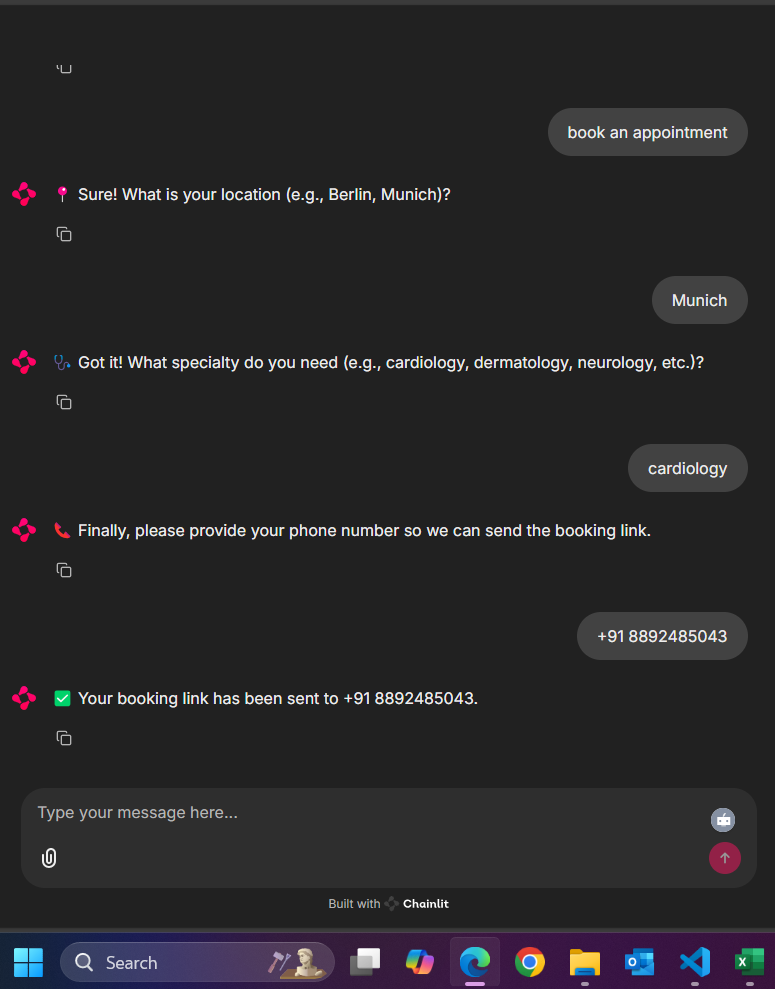
\includegraphics[width=0.85\textwidth]{Images/doclink1.png}
    \caption{A patient booking an appointment. The chatbot requests the location (e.g., Munich) and the specialty (e.g., Cardiology), then collects the user’s phone number to send a booking link.}
    \label{fig:book-appointment}
\end{figure}

As shown in Figure~\ref{fig:book-appointment}, the chatbot confirms the patient’s location and medical specialty. Once the user provides a phone number, the system sends a direct link for appointment scheduling, thereby streamlining the booking process.

\section{Student Role: Medical Explanations}
\label{sec:student-role}


\begin{figure}[htbp]
    \centering
    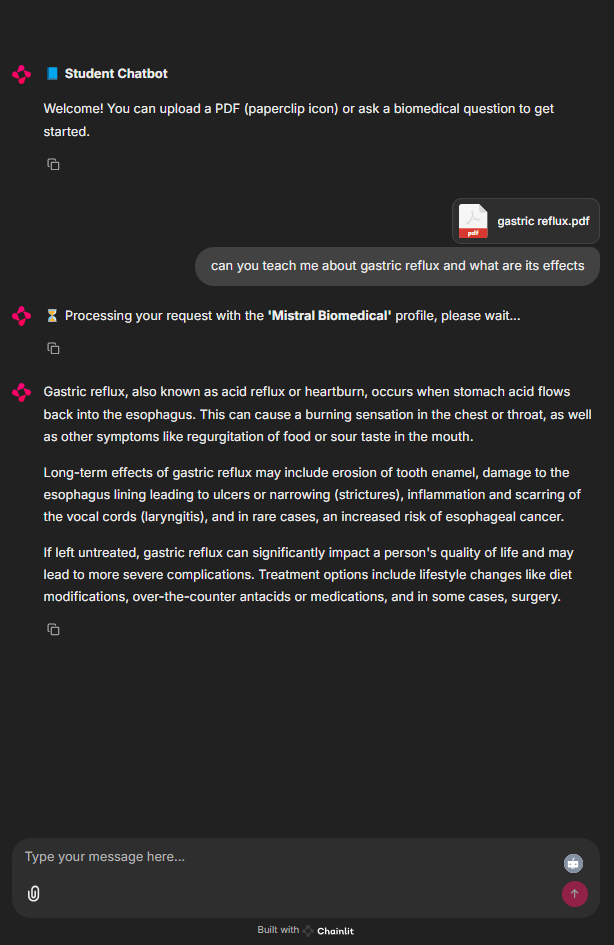
\includegraphics[width=0.85\textwidth]{Images/pdfquestion.png}
    \caption{A student asking for detailed medical information. The chatbot provides an academic explanation suited for learning, referencing embedded content.}
    \label{fig:student-chatbot}
\end{figure}

Figure~\ref{fig:student-chatbot} highlights how a user with the \emph{Student} role can request deeper, evidence-based information. The chatbot uses context from embedded academic texts, ensuring that explanations remain precise and pedagogically useful.

\section{Symptom Analysis and Guidance}
\label{sec:patient-symptoms}

\begin{figure}[htbp]
    \centering
    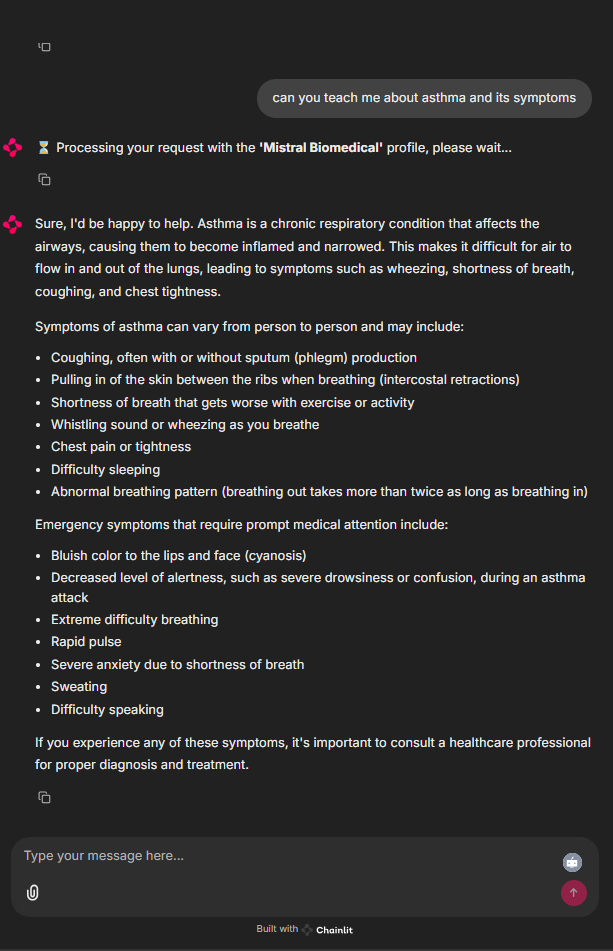
\includegraphics[width=0.85\textwidth]{Images/stuentquestion.png}
    \caption{A student asking specific medical questions (e.g., asthma-related issues) in order to learn more. The chatbot responds with context-aware guidance, referencing standard medical guidelines and educational sources.}
    \label{fig:patient-symptoms}
\end{figure}

In Figure~\ref{fig:patient-symptoms}, a patient reports respiratory symptoms. The chatbot, using retrieval-augmented generation (RAG), provides relevant medical guidance while filtering out any sensitive data at the edge to maintain privacy compliance.

\section{Managing Gastrointestinal Issues}
\label{sec:diarrhea-question}

\begin{figure}[htbp]
    \centering
    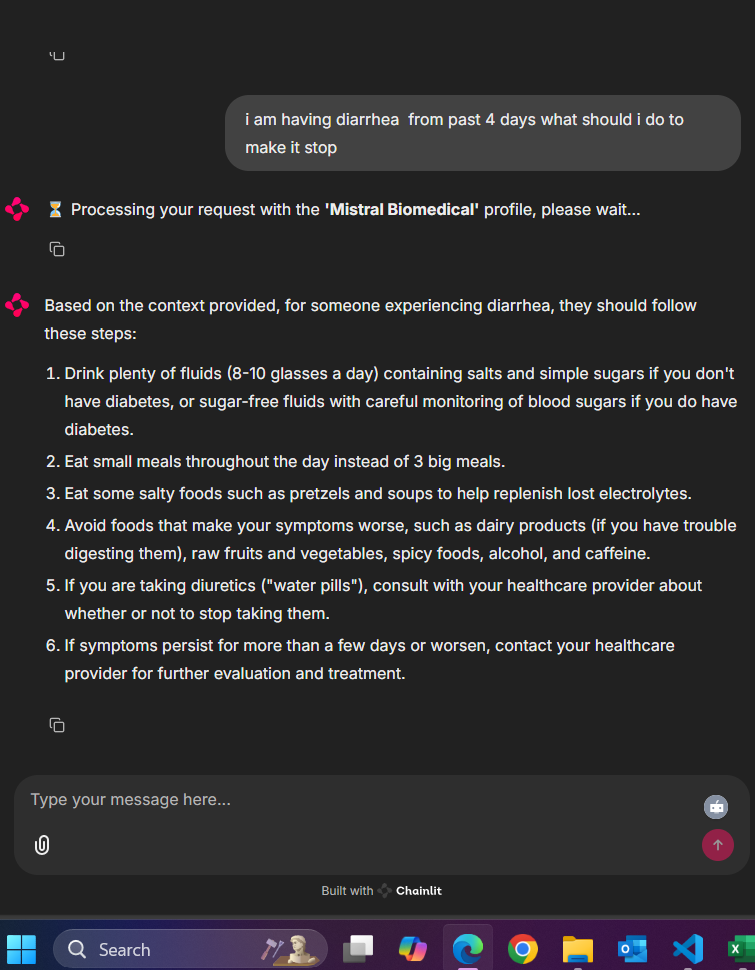
\includegraphics[width=0.85\textwidth]{Images/patientsymptoms.png}
    \caption{A patient scenario discussing diarrhea symptoms for four days. The chatbot suggests dietary measures and advises contacting a healthcare professional if symptoms worsen.}
    \label{fig:diarrhea-question}
\end{figure}

Figure~\ref{fig:diarrhea-question} demonstrates how the chatbot uses user inputs (e.g., “four days of diarrhea”) to provide context-appropriate advice, such as recommending fluid intake and dietary modifications. The system also cautions the user to consult a professional if conditions do not improve.

\section{Provider Recommendations}
\label{sec:doctor-recommendations}

\begin{figure}[htbp]
    \centering
    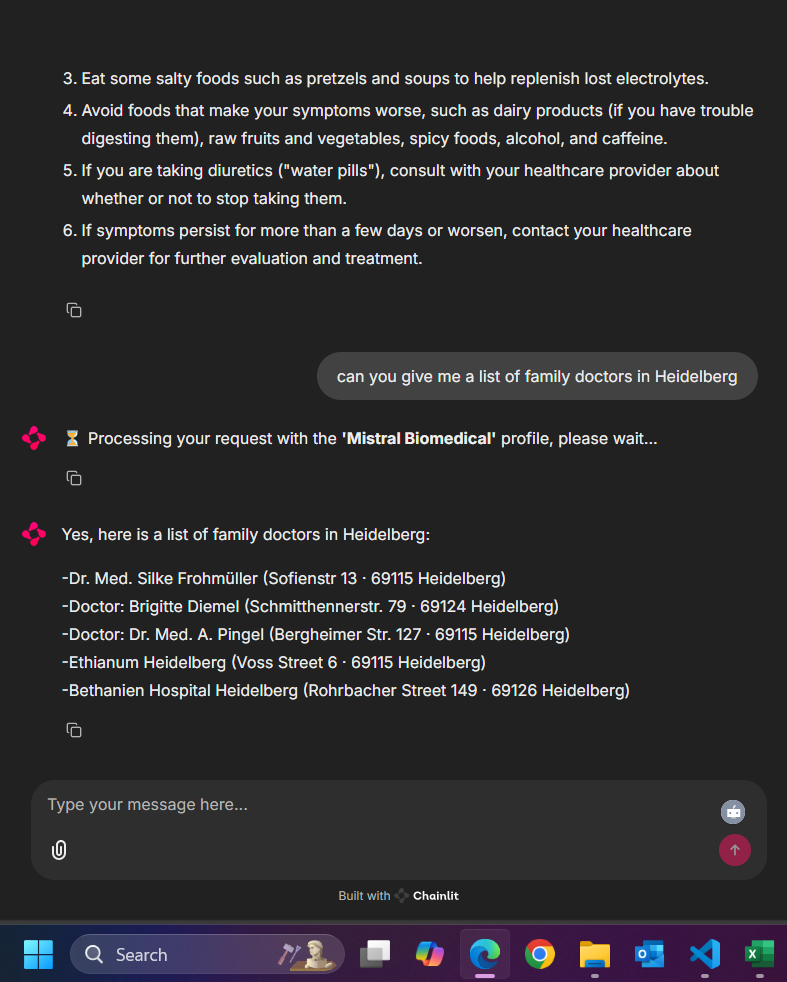
\includegraphics[width=0.85\textwidth]{Images/doctorrecom.png}
    \caption{Chatbot suggesting a list of nearby family doctors in Heidelberg, filtered by location and specialty.}
    \label{fig:doctor-recom}
\end{figure}
In Figure~\ref{fig:doctor-recom}, the chatbot generates a list of nearby healthcare providers based on the patient’s location. This feature demonstrates the system’s ability to integrate location-based data with a specialty filter, simplifying the referral process.


\section{Agentic Booking System}

\begin{figure}[H]
  \centering
  
\includegraphics[width=0.3\textwidth]{Images/appointmentlink.png}
  \caption{Agentic AI demonstration: The system automatically integrates with Twilio 
    to send the user an appointment booking link for a cardiology specialist in Munich.}
  \label{fig:agentic_ai_booking}
\end{figure}

\section{Discussion of Chatbot Interaction Results}
Overall, these screenshots illustrate the chatbot’s capacity to:
\begin{itemize}
    \item \textbf{Identify user roles} (patient vs.\ student) and deliver tailored content.
    \item \textbf{Provide medical insights} based on retrieval-augmented generation (RAG).
    \item \textbf{Offer practical guidance} such as appointment booking and provider recommendations.
\end{itemize}

These functionalities address the research questions outlined in the earlier chapters, showcasing how the system can effectively serve both educational and clinical needs in a unified platform.

 
\chapter{Conclusion and Future Work}

\label{Chapter6}

\lhead{Chapter 6. \emph{Conclusion and Future Work}}

This final chapter of the thesis serves to conclude the research, by presenting a comprehensive reflection on the various aspects explored and identifies potential 
areas for the future research. This chapter will give an quick overview of the thesis by providing  the key findings, conclusion and future work. As the main
objective of this thesis is to identify an unique approach which can handle the complex relationships among sentences in a text and to achieve the 
topic modelingusing the latest techniques.

%%%%%%%%%%%%%%%%%%%%%%%%%%%%%%%%%%%%%%%%%%%%%%
% section : Conclusion
%%%%%%%%%%%%%%%%%%%%%%%%%%%%%%%%%%%%%%%%%%%%%%
\section{Conclusion}

This thesis proposes a new method of topic modeling, unlike the earlier methods in the forms of LDA, NMF, and LSA. 
The conventional approaches have great capabilities in topic extraction, but they still strongly depend on word co-occurrence patterns.
 Besides, they cannot extract the deeper contextual understanding of text data. Meanwhile, BERTopic is a language model-based topic modeling 
 that covers an alternative by making use of embeddings, dimensionality reduction, clustering, and the representation of topics using c-TF-IDF and count 
vectorizer techniques. Despite such merits, at the same time, BERTopic fails in completely capturing such complex semantic relationships among words in
 a text. Moreover, performance can be poor for smaller datasets, and results may slightly vary on runs with the same data.

Considering these limitations, a new approach to topic modeling in an attempt to solve some of these challenges.
In particular, this thesis focuses on improving topic modeling by providing better semantic understanding of relationships 
among sentences and extracting more meaningful topics from text. While the novelty of this approach embeds, reduces the
dimensionality, and clusters, it makes a further step by feeding the clustered sentences into large language models. 
Large language models are better equipped to grasp complex semantic relationships and therefore allow for more 
accurate and insightful topic generation. This, in turn, helps the researchers and analysts in identifying the 
underlying themes and patterns in text data more appropriately.

As the dataset is in German language, choosing the right embeddings model is a very important part of the process to get the best results.
There are many embeddings models which can be used to tackle the problem but, I chose Jina embedding-v2-base-de model because of its 
capabilities to handle both English and German languages data and gave better clustering results than other models and it 
uses less computational power and time to process the data. For clustering the embedded data, I have used HDBSCAN algorithm over K-Means
as it struggles to handle noise in the data and also need to specify the number of clusters in advance.
As the language models are powerful in extracting the semantic relationships and most of the models are multilingual and handle German
language feeding the clustered sentences to LLMs model will help to extract more meaningful topics for the text documents.

%%%%%%%%%%%%%%%%%%%%%%%%%%%%%%%%%%%%%%%%%%%%%%
%section : answers to research questions
%%%%%%%%%%%%%%%%%%%%%%%%%%%%%%%%%%%%%%%%%%%%%%
\section{Answers to Research Questions}

By answering the research questions that were formed earlier in this thesis, we shall be able to appreciate its possibilities and whether its objectives have been met.
\begin{enumerate}
    \item\textbf{Q1: How does topic modelling aid in the extraction of topic process from the dataset of past interviews?}
    
    The topic modelling approach can be used to extract the topics from the historical interview dataset as this question was made to understand the topic which were already 
    exsited in the past to understand how the topic modeling has been achieved in the past and how it can be improved. This question help to understand the potential of the approaches
    like LDA, NMF, LSA, BERTopic, prompt-topic-model etc., and how they can be improved in the past to achieve better results. With the help of this question, I was able to understand 
    the workflow which has been used and about its advantages and disadvantages and how has been used in the past which various approaches to achieve better results. This question
    helped me to understand the potential of the approaches and how it can be used for the interview dataset. This question also helped me to come up the idea of approaching the 
    problem of handling the huge text data by using embedding, clustering and use of large language models.
    
    \vspace{0.3cm}
    \item\textbf{Q2: How can we use various clustering techniques to extract information and cluster them from the German dataset?}
    
    This question will help me to understand the various clustering techniques and how they can be used to in this thesis to achieve topic modelling. There are many clustering techniques
    like K-Means, DBSCAN, Hierarchical Clustering, HDBSCAN etc., which will help to cluster the data. This research support for choosing the clustering technique suitable for the dataset.
    As these techniques are effective in grouping the data which are similar to each other. After understnading the pros and cons of various clustering techniques, which helped to achieve
    better cluster formation for the text data in this thesis. As the number of topics present in the data is unknow and identifying the topics from the data is difficult this question helped
    to understand how clustering techniques can be used to achieve the topic modelling. After understanding the various aspects of clustering algorithms, this question helped me to choose
    the HDBSCAN algorithm to achieve better results. As this algorithm is effective in group the similar data point to each other, it can handle the noise in the data and it also doesn't 
    require specifying the number of clusters in advance.
    
    \vspace{0.3cm}
    \item\textbf{Q3: How can language models be applied for topic modelling of German datasets?}
    
    This question was asked in order to know how the language models can be applied to the German dataset. As well all know about the language models and how powerfull they are can be used
    used for multilingual and cross lingual applications. So, the language models can be used for the German language datasets. However, to achieve topic modelling through language models
    is not an easy task. As the LLM model can't be used to directly extract the topic from the data and this processing of large amount of data cannot be handled by LLM model. So, this question
    helped to understand the potential of the approaches and as mention in research question 1, about the thesis approach where the data will undergoes embedding and clustering then, the clustered 
    data will be fed to LLM model through the prompt to generate the topic names. In this way the LLM model can be used to extract the topic from the huge dataset. There are many advantages of using the
    LLM model to extract the topic when compare to traditional approaches, as the traditional methods will extarct the topic based on the occurrence of the words in the data but, the LLM model
    can understand the context of the sentences in the cluster and generate the topic names. There are many open source LLm model available and can be used based on the computational power of the device.

\end{enumerate}

%%%%%%%%%%%%%%%%%%%%%%%%%%%%%%%%%%%%%%%%%%%%%%
%section : future work and challenges
%%%%%%%%%%%%%%%%%%%%%%%%%%%%%%%%%%%%%%%%%%%%%%
\section{Future Work and Challenges}

The methods used in this thesis were effective for extracting the topics from the historical interview transcripts along with the corresponding
challenges. Firstly, the noise present in the datast can be managed in much better way. The noise are not removed completely which is ending up in 
forming a seperate cluster which is full of noise. Secondly, with the limited available of the computational power is major challenge 
faced as the embedding model and language model needs high computational power to process the data. 
Latest version of LLMs were not used due to the high computational power. 
Thridly, handling of the noise in the data, as the removal stopwords and normalizing the data will have higher chance of losing the context of the
information. Hence, the small amount of noise has been removed after looking into the cluster results but, the noise are not removed completely.

In Future, with the help of better computational resources the challenges of using bigger and better embedding models and language models can be utilized
for even better results. The prompting to the language models can be improved which will result in better topic name generation.
Hyperparameters can be fine-tuned to get even better results. The web application can also be improved by using the better UI design and better styling.



%----------------------------------------------------------------------------------------
%	THESIS CONTENT - APPENDICES
%----------------------------------------------------------------------------------------

\addtocontents{toc}{\vspace{1em}} % Add a gap in the Contents, for aesthetics

\appendix % Cue to tell LaTeX that the following 'chapters' are Appendices

 %Appendix A
\chapter{Source Code} % Main appendix title
\label{Source Code} % For referencing this appendix elsewhere, use \ref{AppendixA}
\lhead{Appendix A:\emph{Source Code}} 


\noindent The Source Code is available on GitHub. 

\noindent\textbf{GitHub Link:} \href{https://github.com/naveen987/Master-Thesis}{https://github.com/naveen987/Master-Thesis}
%\input{Appendices/AppendixB}
%\input{Appendices/AppendixC}

\addtocontents{toc}{\vspace{1em}} % Add a gap in the Contents, for aesthetics

\backmatter

%----------------------------------------------------------------------------------------
%	BIBLIOGRAPHY
%----------------------------------------------------------------------------------------

\label{Bibliography}

\lhead{\emph{Bibliography}} % Change the page header to say "Bibliography"

\bibliographystyle{apalike}  
\bibliography{bibliography.bib}
%\bibliographystyle{apalike} % Use the "apalike" BibTeX style for formatting the Bibliography

%\bibliography{bibliography} % The references (bibliography) information are stored in the file named "bibliography.bib"

\end{document}
